\chapter{Dane i zmienne}
\label{ch:dane}

\section{Opis zbioru danych}
Dane odgrywają kluczową rolę w analizie i prognozowaniu cen energii na Rynku Dnia Następnego (RDN) w Polsce, stanowiąc fundament dla modeli uczenia maszynowego zastosowanych w niniejszej pracy. Zbiór danych wykorzystany w badaniu obejmuje okres od 1 stycznia 2016 roku do 31 grudnia 2024 roku i zawiera dane godzinowe, co powinno było dać łącznie 78 912 rekordów. Niestety niektóre dane są niekompletne i zawiera braki lub NaN wartości. Na szczęście, takich braków było stosunkowo nie dużo do kompletnych danych i postanowiłem pozbyć się rekordów o pustych parametrach. W efekcie, po usunięciu niekompletnych danych, pozostało 78 814 rekordów, co stanowi solidną podstawę do analizy i modelowania. Zbiór danych zawiera różnorodne zmienne, które można podzielić na kilka kategorii, które zostaną opisane w tym dziale. Większość danych pochodzi z \gls{pse} \cite{PSEOLD}, czyli otwartej platformie, która dostarcza różnego rodzaju danych dostępnych dla analizy. Warto zauważyć, że od 14 czerwca 2024 roku PSE zmieniła sposób raportowania danych i przeszła na nową stronę \cite{PSENEW}, w związku z tym PSE posiada dwie oddzielne strony do raportów historycznych przed i po tym dniu. Wiele z danych zostały pobrane również ze strony energy.instrat.pl. Jest to strona, która pobiera dane z platformy PSE i udostępnia w sposób wygodniejszy, ponieważ dane są do pobrania jednym klikiem za dowolny okres czasu z dowolną częstotliwością. Dane dotyczące cen paliw kopalnych oraz kursów walut (np. PLN/USD) zostały pozyskane z innych źródeł, takich jak publiczne bazy danych rynkowych i platformy finansowe. Niniejszy rozdział szczegółowo opisuje zmienną zależną i zmienne niezależne, podzielone na kategorie, a także prezentuje kluczowe cechy danych za pomocą tabel i wykresów, co pozwala na lepsze zrozumienie ich specyfiki i wyzwań związanych z modelowaniem.

\section{Zmienna zależna}
Zmienna zależna w niniejszej pracy to fixing\_i\_price, czyli cena energii elektrycznej na Rynku Dnia Następnego (RDN) w Polsce, wyrażona w PLN/MWh. Dane dotyczące tej zmiennej zostały pobrane z wymienionej platformy energy.instrat.pl w granulacji godzinowej. Zbiór danych obejmuje okres od 1 stycznia 2016 roku do 31 grudnia 2024 roku. Statystyki opisowe zmiennej fixing\_i\_price przedstawiono w Tabeli poniżej. 
\begin{table}[H]
    \centering
    \begin{tabular}{|l|r|}
    \hline
    \textbf{Statystyka} & \textbf{Wartość} \\ \hline
    Średnia             & 344.10 PLN/MWh   \\ \hline
    Odchylenie std.     & 268.35 PLN/MWh   \\ \hline
    Minimum             & -360.00 PLN/MWh  \\ \hline
    25\% (Q1)           & 176.11 PLN/MWh   \\ \hline
    Mediana             & 250.00 PLN/MWh   \\ \hline
    75\% (Q3)           & 434.84 PLN/MWh   \\ \hline
    Maksimum            & 3812.45 PLN/MWh  \\ \hline
    \end{tabular}
    \caption{Podstawowe statystyki zmiennej fixing\_i\_price}
    \label{tab:fixing-i-price-stats}
\end{table}

Aby lepiej zrozumieć dynamikę cen energii na RDN, przeanalizowano ich zmienność w całym okresie badania. Rysunek poniżej przedstawia zmienność cen energii w czasie zebranych danych.

\begin{figure}[H]
    \centering
    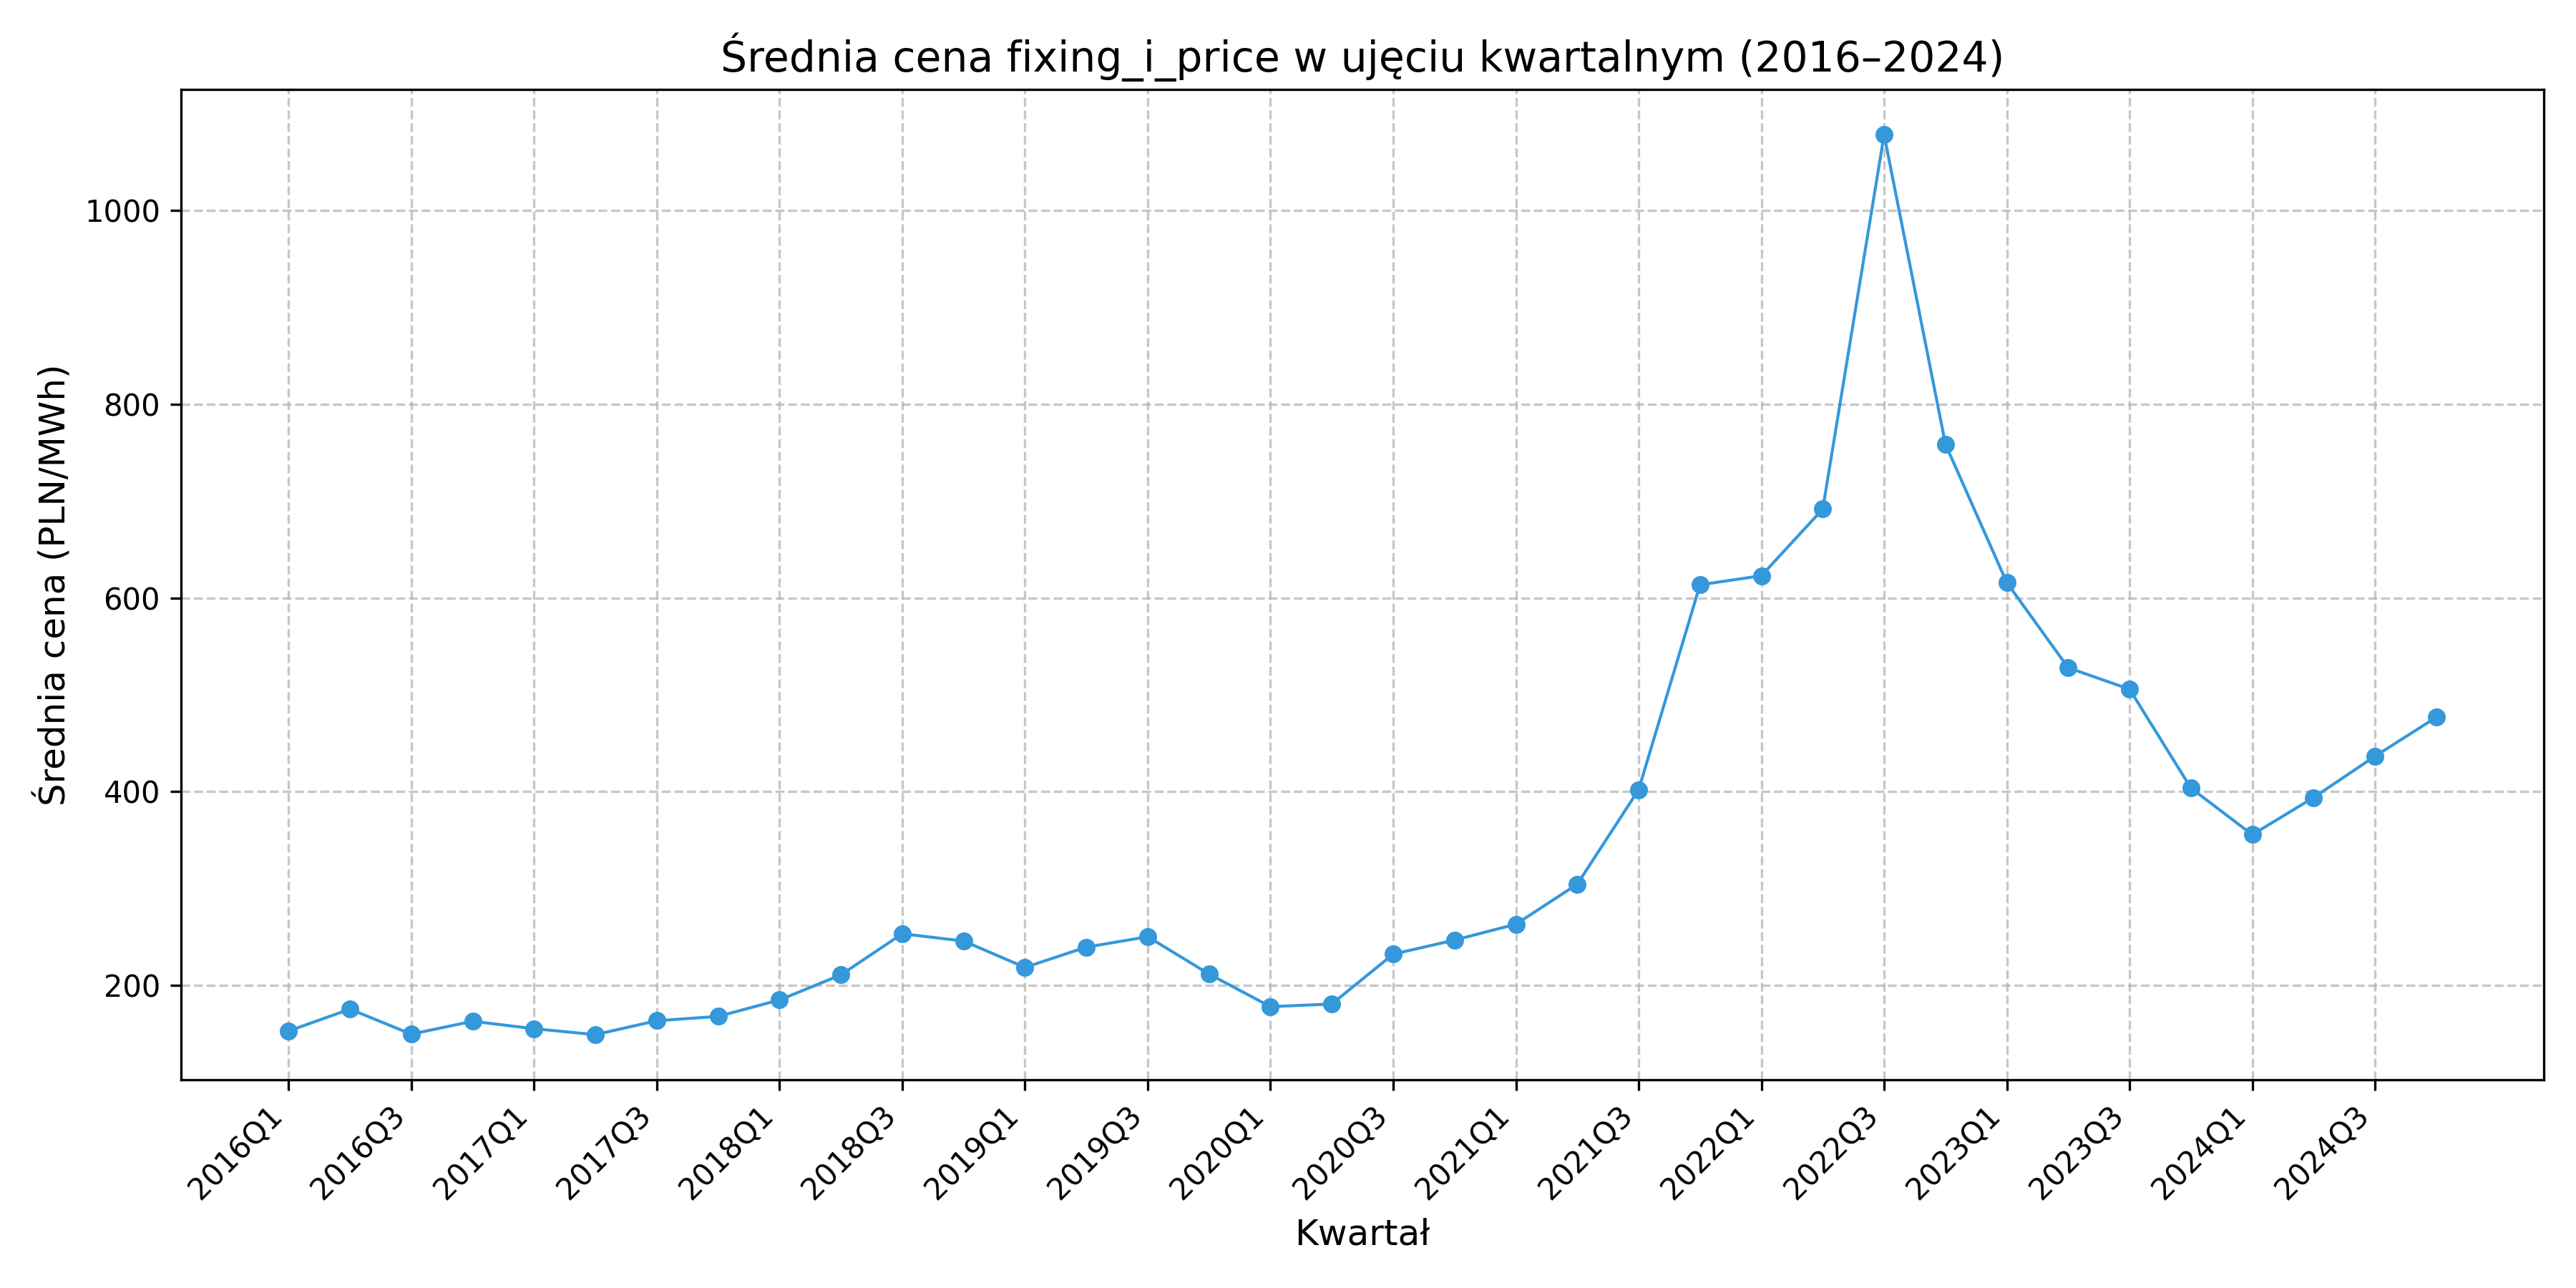
\includegraphics[width=\textwidth]{../plots/data/quarterly_fixing_i_price.png}
    \caption{Zmienność cen energii elektrycznej na RDN w latach 2016–2024}
    \label{fig:fixing-i-price-trend}
\end{figure}

Widać wyraźne różnice w poziomie cen w różnych okresach: od 2016 do Q4 roku 2020 ceny były stosunkowo stabilne, oscylując w przedziale 100–300 PLN/MWh. Sytuacja zmieniła się w 2020 roku, gdy zaczęły pojawiać się pierwsze skoki cenowe z powodu poważnych obostrzeń z powodu pandemii, a w 2022 roku, w wyniku kryzysu energetycznego wywołanego wojną na Ukrainie i ograniczeniami w dostawach paliw kopalnych, ceny osiągnęły rekordowe poziomy. Pierwszy okres zostanie określony jako okres stabilności cenowej, a drugi jako okres skoków cenowych. Te dwa okresy pokazują, jak niekorzystne sytuacje gospodarcze mogą wpływać na dynamikę cen energii, co ma istotne implikacje dla modelowania i prognozowania.

\begin{figure}
    \centering
    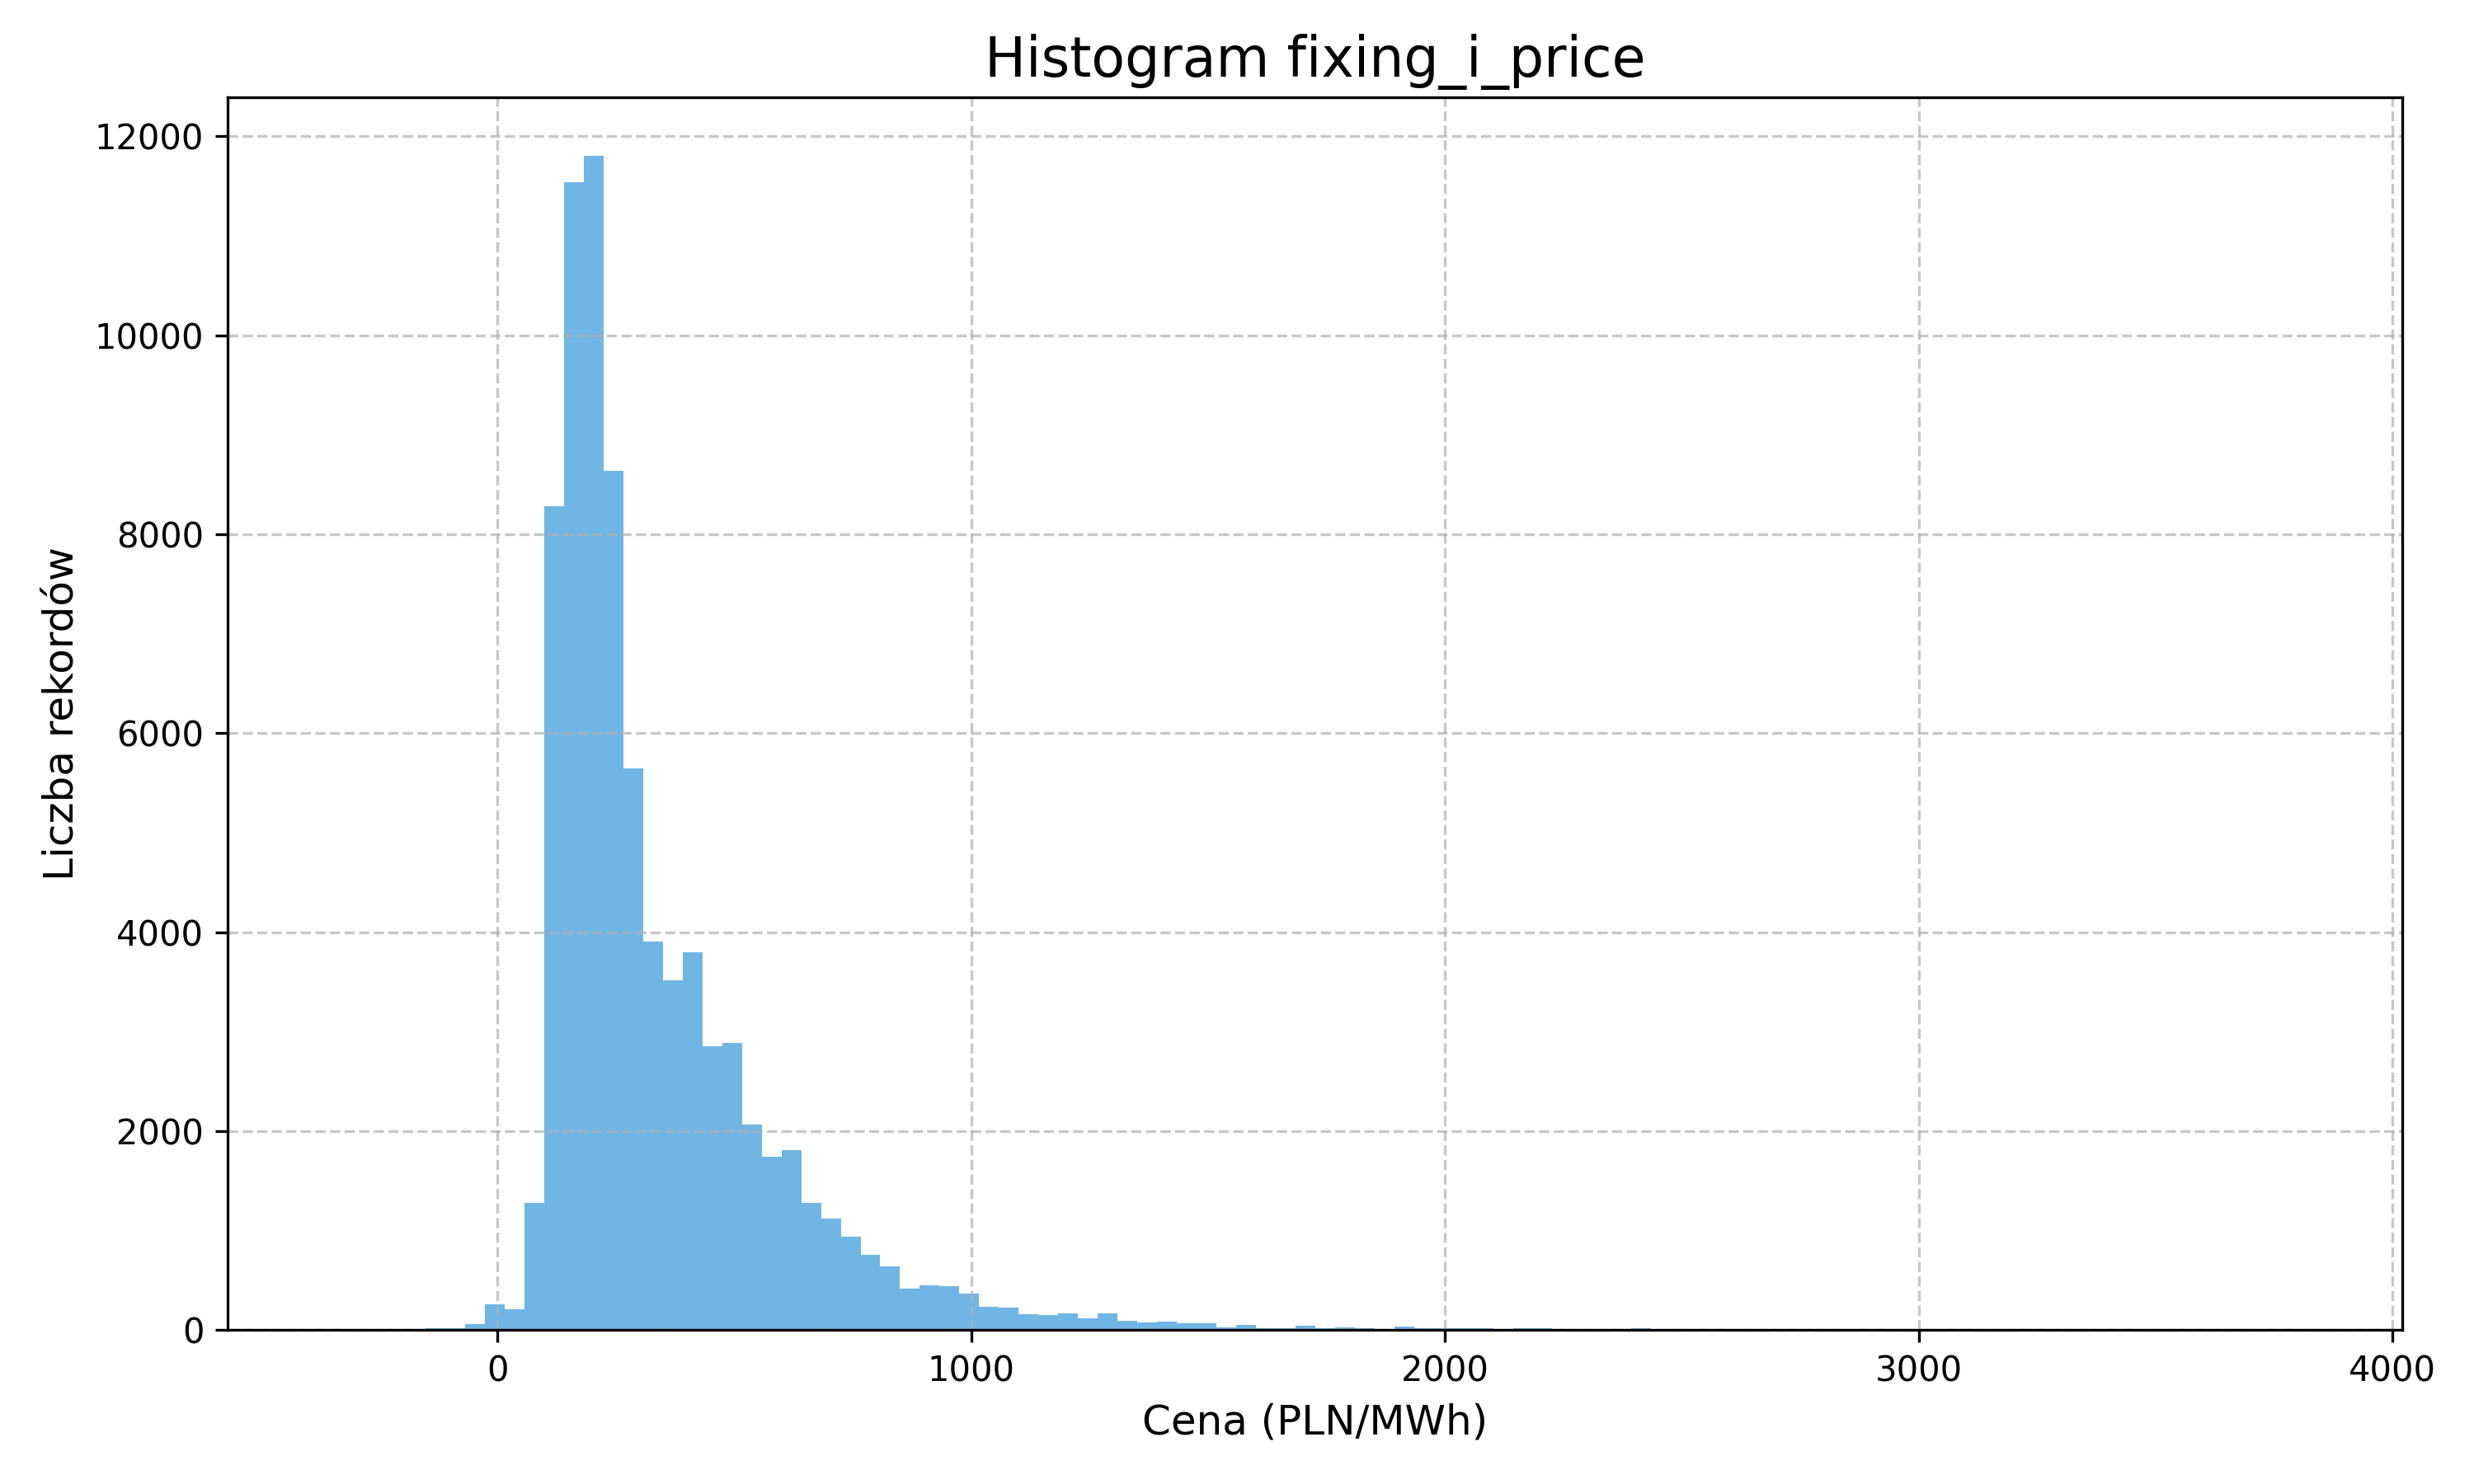
\includegraphics[width=\textwidth]{../plots/data/histogram_fixing_i_price.png}
    \caption{Histogram rozkładu zmiennej fixing\_i\_price}
    \label{fig:fixing-i-price-histogram}
\end{figure}

Rysunek \ref{fig:fixing-i-price-histogram} przedstawia histogram rozkładu zmiennej \texttt{fixing\_i\_price}. Rozkład jest wyraźnie asymetryczny, z długim prawym ogonem, co odzwierciedla występowanie skoków cenowych, takich jak te w 2022 roku. Ujemne ceny, choć rzadkie (ok. 0,4\% rekordów), są widoczne w lewej części histogramu, co potwierdza specyficzne cechy danych i potrzebę stosowania odpowiednich metod modelowania.

\section{Zbiór zmiennych niezależnych}
Dobór zmiennych niezależnych jest bardzo ważny dla osiągnięcia dobrych wyników badania. W niniejszej pracy wykorzystano różnorodne zmienne niezależne, które można podzielić na kilka kategorii. Obejmują one dane pogodowe, zapotrzebowanie, straty sieciowe, bilanse wymiany transgranicznej, dane o produkcji energii przez poszczególne typy generatorów, ceny paliw kopalnych, emisji CO$_2$ i inne. Wybór tych zmiennych oparty jest na ich potencjalnym wpływie na ceny energii elektrycznej. Poniżej przedstawiono szczegółowy opis każdej z kategorii zmiennych niezależnych, które zostały uwzględnione w analizie.

\subsection{Dane pogodowe}
Pierwotnie zbiór danych miał być zestawiony z danych dostępnych za pomocą oficjalnej strony Instytutu Meteorologii i Gospodarki Wodnej, natomiat dane historyczne z lat 2016-2024 mają ograniczoną rozdzielczość. Zbierane są przez wiele stacji meteorologicznych, które są rozproszone po całym kraju, ale tylko w godzinach 6:00, 12:00 oraz 18:00. Aproksymować dane pogodowe w godzinach nocnych jest zadaniem nie do wykonania, szczególnie w przypadku sezonów zimowych, gdzie temperatura w nocy może drastycznie spadać w ciągu godziny. Z tego powodu jako źródło danych pogodowych wykorzystano stronę open-meteo.com \cite{METEO}. Jest to strona, która zbiera dane z różnych stacji meteorologicznych i udostępnia je w formie API. Dzięki temu można pobrać dane pogodowe dla dowolnego okresu czasu i lokalizacji.

Dane pogodowe zostały pobrane dla czterech lokalizacji w Polsce: Warszawy (WAW), Koszalina (KSZ), Krakowa (KRK) i Babimost (BAB), a następnie dopasowane do godzinowego formatu danych RDN, co pozwoliło na ich integrację z pozostałymi zmiennymi. Wybór miast został podyktowany ich zróżnicowaniem geograficznym i klimatycznym, co pozwala uwzględnić regionalne różnice w warunkach pogodowych wpływających na produkcję i zapotrzebowanie na energię. Warszawa, jako stolica i największe miasto Polski, reprezentuje centralny region kraju o wysokim zapotrzebowaniu na energię, szczególnie w okresach zimowych i letnich. Koszalin, położony na Pomorzu, jest kluczowy ze względu na bliskość farm wiatrowych na Morzu Bałtyckim, co czyni go istotnym punktem dla analizy produkcji energii wiatrowej. Kraków, znajdujący się w południowej Polsce, charakteryzuje się większym udziałem energii słonecznej w miksie energetycznym, a także wysokim zapotrzebowaniem na energię w sezonie grzewczym z powodu zanieczyszczenia powietrza i częstego stosowania ogrzewania elektrycznego. Babimost, zlokalizowany w zachodniej Polsce, jest istotny ze względu na swoje położenie w pobliżu granicy z Niemcami.

Parametry pogodowe zostały wybrane z uwzględnieniem ich bezpośredniego wpływu na rynek energii. Temperatura jest kluczowym czynnikiem, ponieważ wpływa na zapotrzebowanie na energię – niskie temperatury zwiększają zużycie energii na ogrzewanie, natomiast wysokie temperatury latem podnoszą zapotrzebowanie na klimatyzację. Prędkość wiatru mierzona na wysokości 100 metrów nad powierzchnią ziemi została wybrana, ponieważ jest to przeciętna wysokość dla turbin wiatrowych w Polsce, co pozwala dokładniej oszacować potencjalną produkcję energii z farm wiatrowych. Promieniowanie słoneczne jest istotne dla produkcji energii z paneli fotowoltaicznych. Zachmurzenie zostało uwzględnione, ponieważ wysoki poziom zachmurzenia zmniejsza efektywność paneli słonecznych, co może zwiększać ceny energii poprzez ograniczenie podaży z OZE. Wybór tych parametrów pozwala na kompleksową analizę wpływu pogody na ceny energii na RDN.

Poniżej przedstawię wykresy dla każdego z parametrów pogodowych, które zostały uwzględnione w analizie. Wykresy przedstawiają zmienność danych pogodowych w czasie. Zachmurzenie jest wyrażone w oktantach (0-8), gdzie 0 oznacza brak zachmurzenia, a 8 oznacza całkowite zachmurzenie.

\begin{figure}[H]
    \centering
    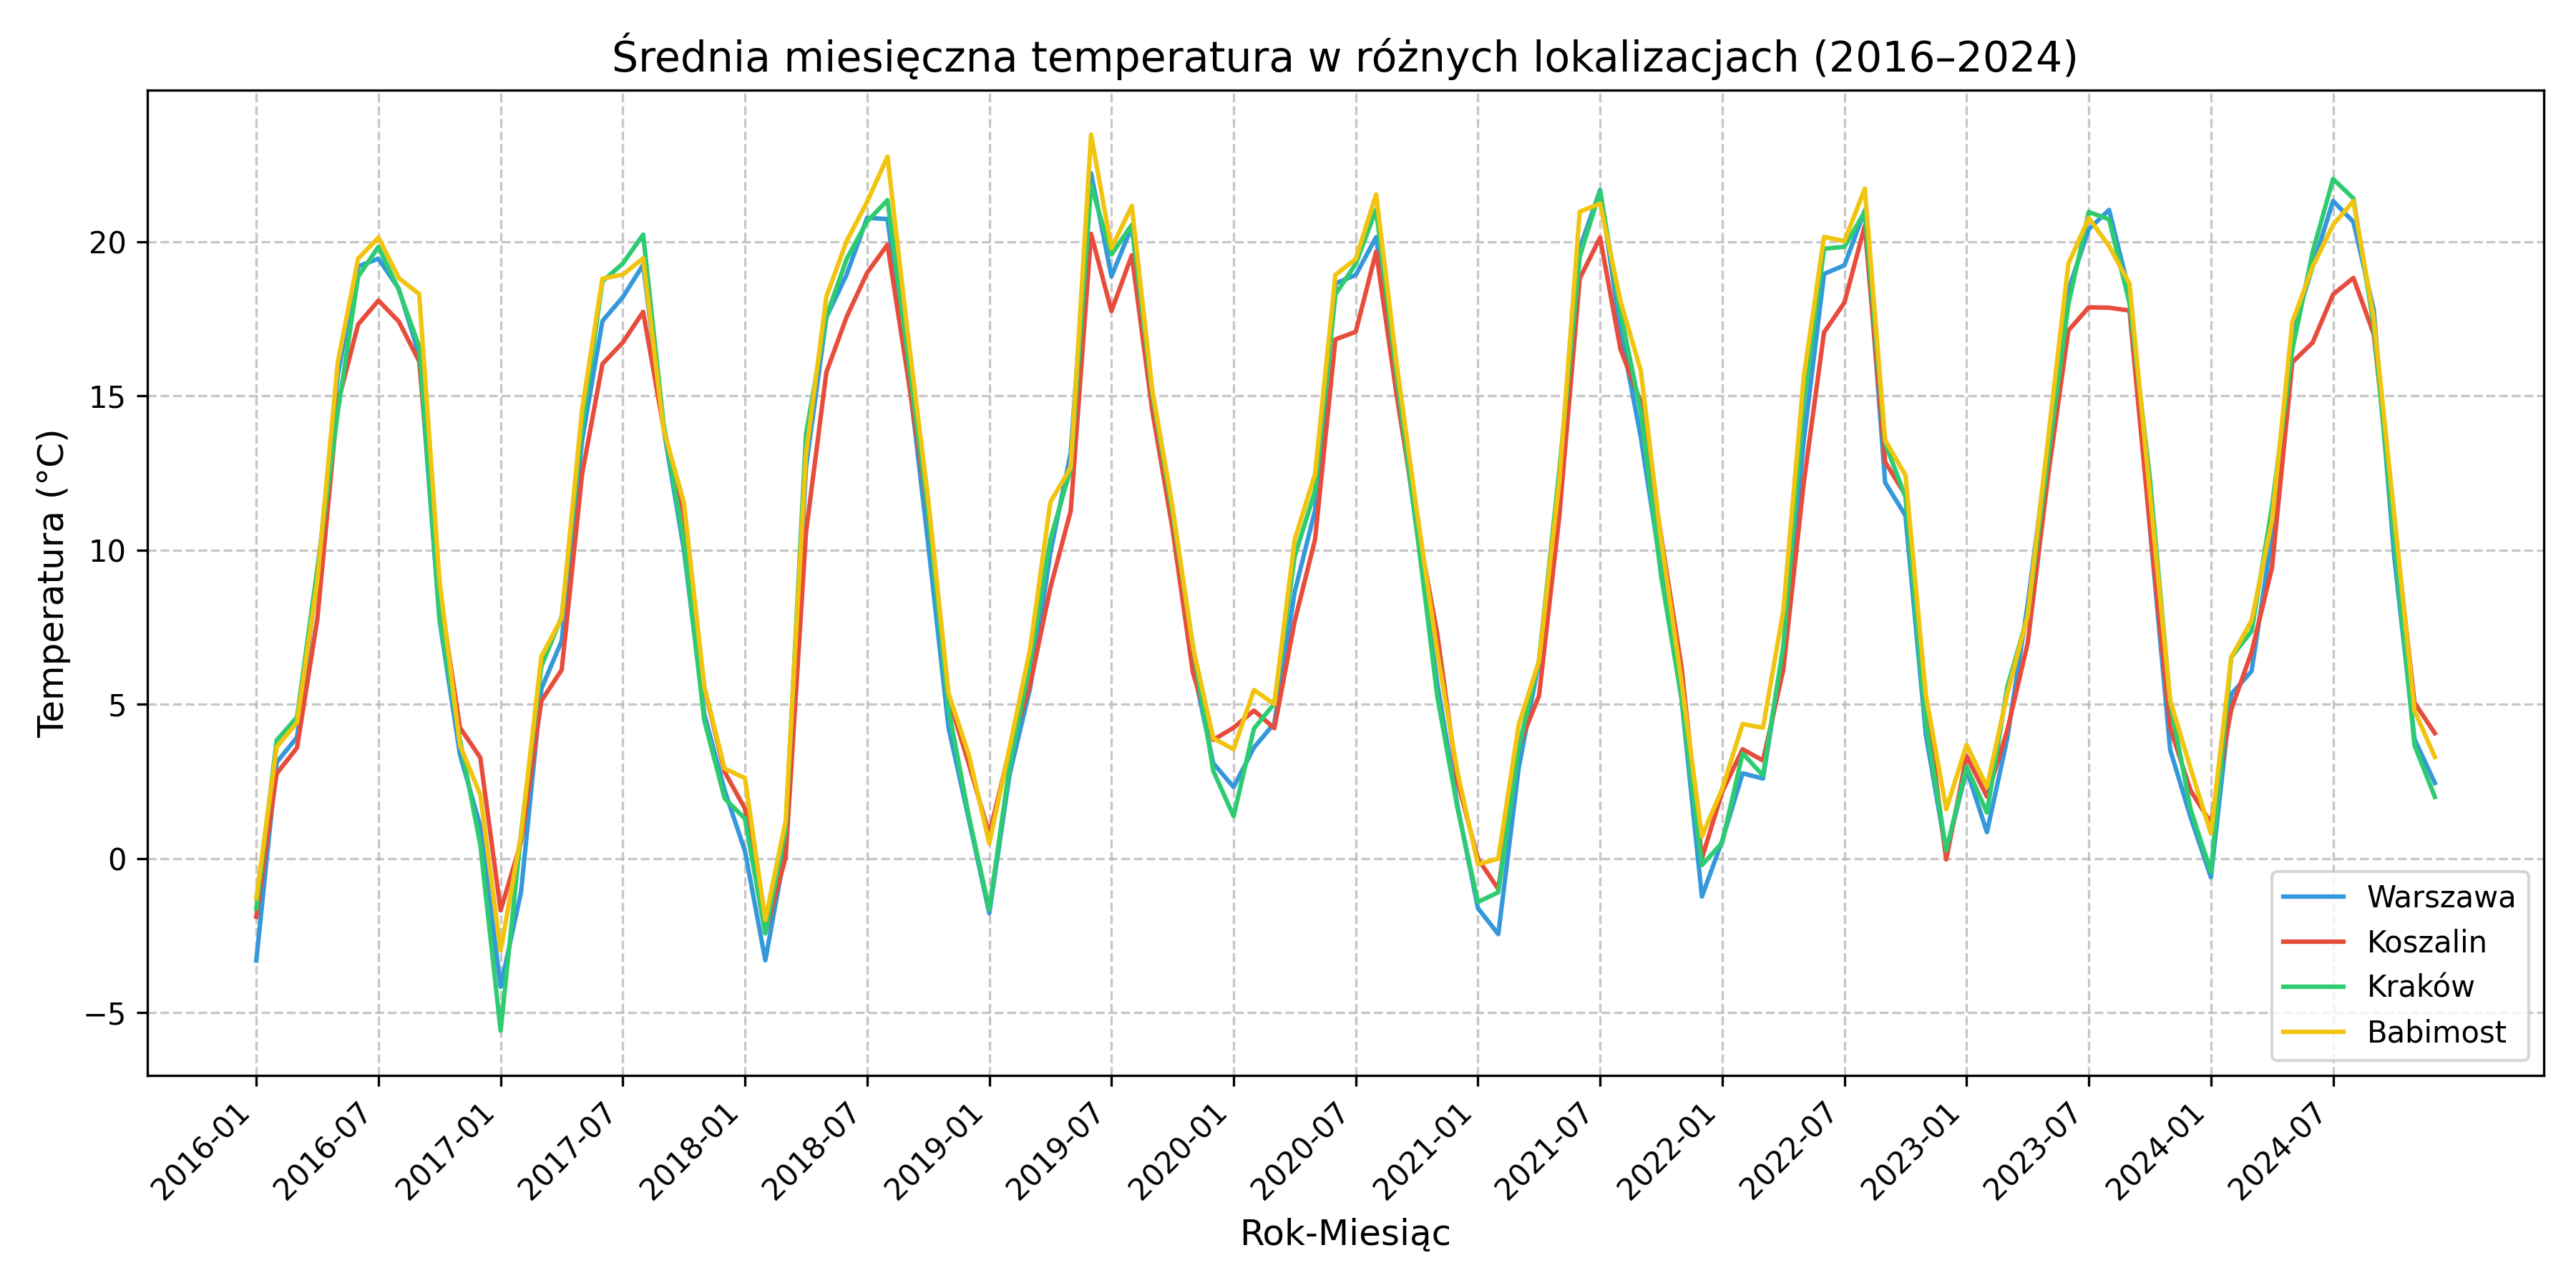
\includegraphics[width=\textwidth]{../plots/data/temp_time_series_full.png}
    \caption{Zmienność temperatury w czasie (2016–2024)}
    \label{fig:temp-time-series-full}
\end{figure}

\begin{figure}[H]
    \centering
    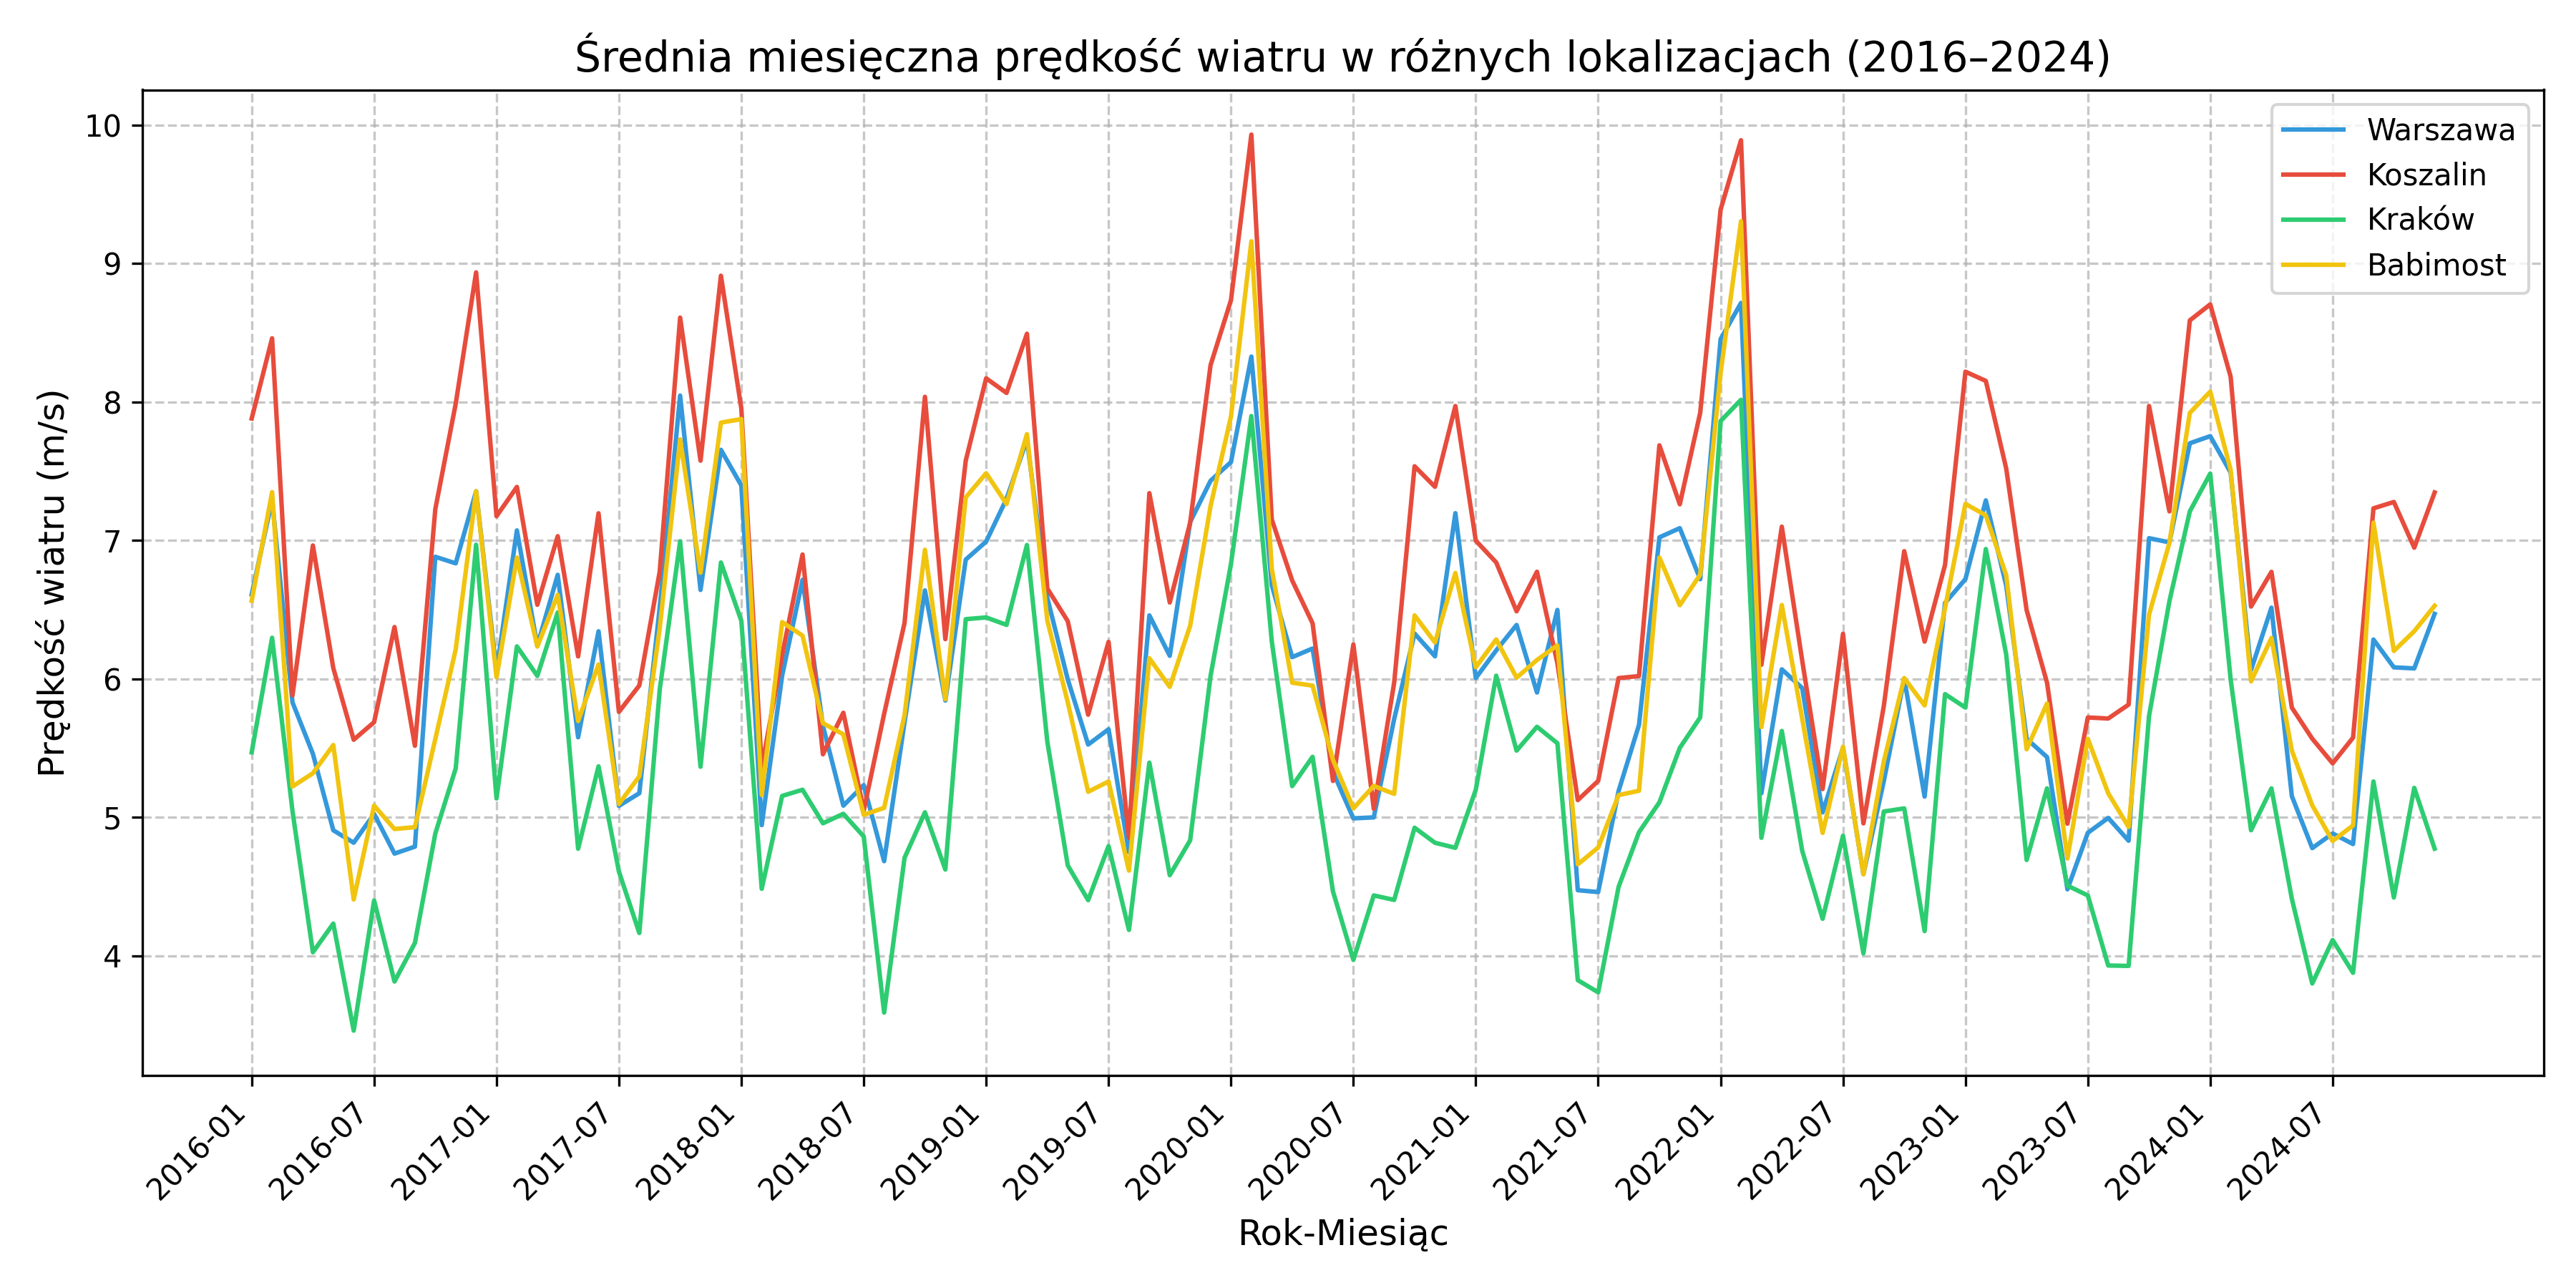
\includegraphics[width=\textwidth]{../plots/data/wind_speed_time_series_full.png}
    \caption{Zmienność prędkości wiatru w czasie (2016–2024)}
    \label{fig:wind-speed-time-series-full}
\end{figure}

\begin{figure}[H]
    \centering
    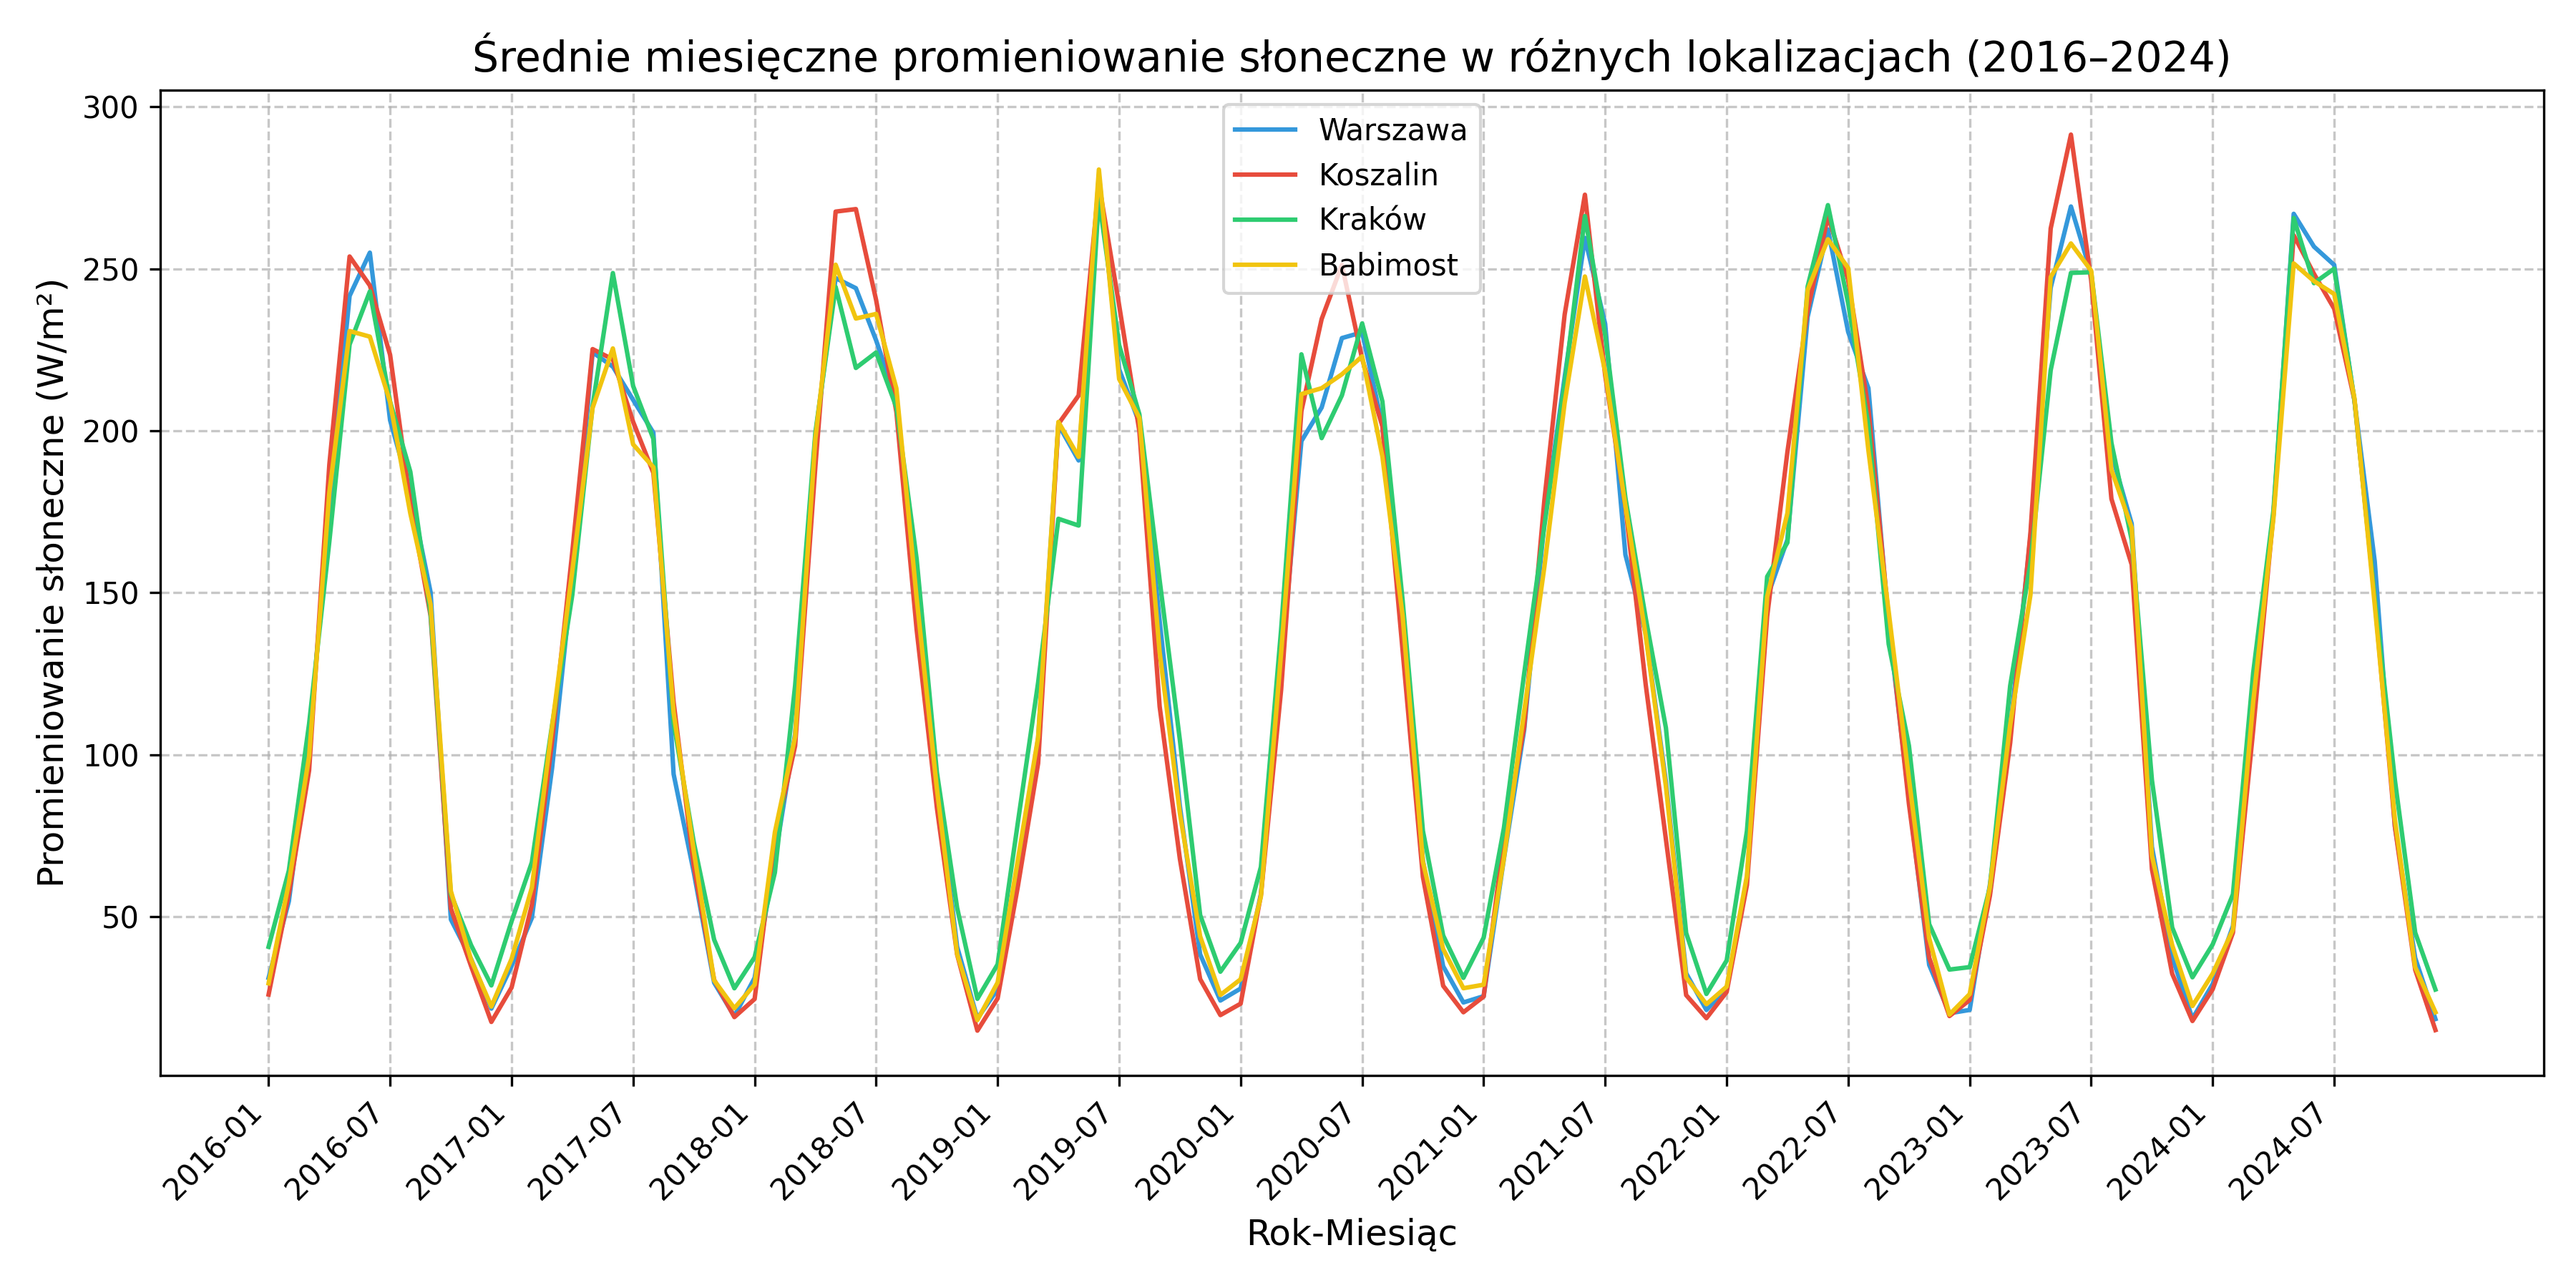
\includegraphics[width=\textwidth]{../plots/data/solar_radiation_time_series_full.png}
    \caption{Zmienność promieniowania słonecznego w czasie (2016–2024)}
    \label{fig:solar-radiation-time-series-full}
\end{figure}

\begin{figure}[H]
    \centering
    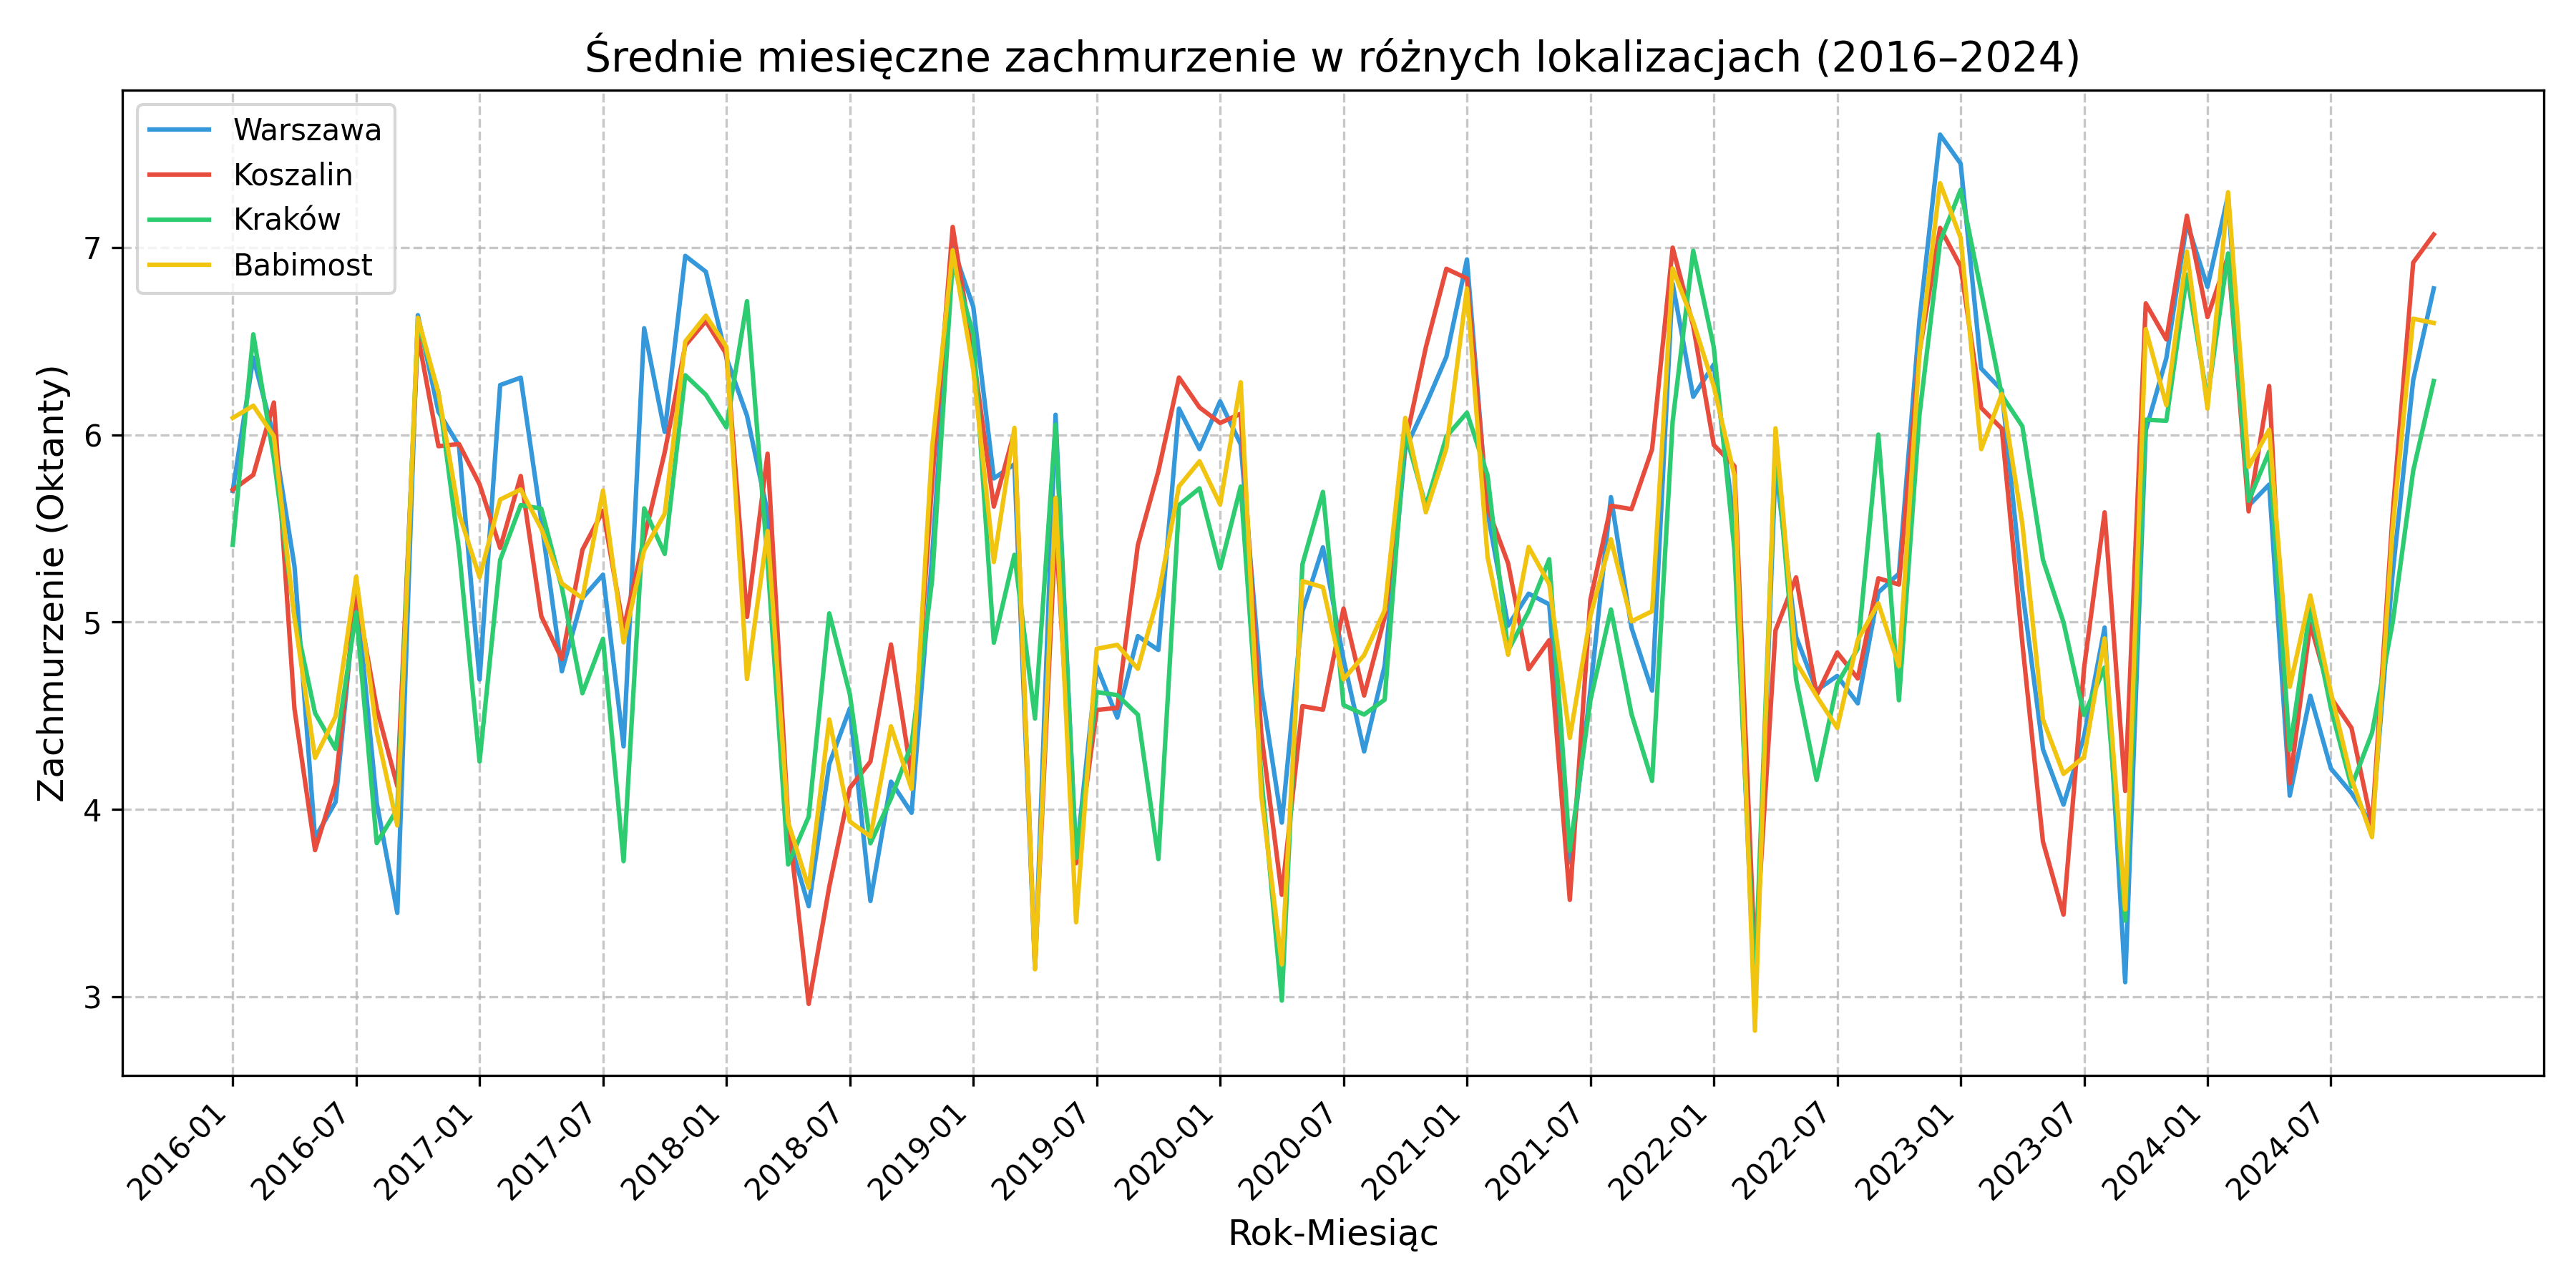
\includegraphics[width=\textwidth]{../plots/data/cloud_cover_time_series_full.png}
    \caption{Zmienność zachmurzenia w czasie (2016–2024)}
    \label{fig:cloud-cover-time-series-full}
\end{figure}

Każdy z wykresów przedstawia zmienność danego parametru pogodowego w wybranych lokalizacjach w przeciągu okresu badawczego. Wyraźnie widać sezonowe wahania parametrów pogodowych, co jest typowe dla klimatu Polski. Temperatura i promieniowanie słoneczne mają wyraźnie większe wartości w sezonach letnich, prędkość wiatru w sezonach zimowych, a zachmurzenie ma bardziej zróżnicowany charakter.

Chciałbym również przybliżyć wykresy i potwierdzić efekt sezonowości na przykładzie 2022 roku. 

\begin{figure}[H]
    \centering
    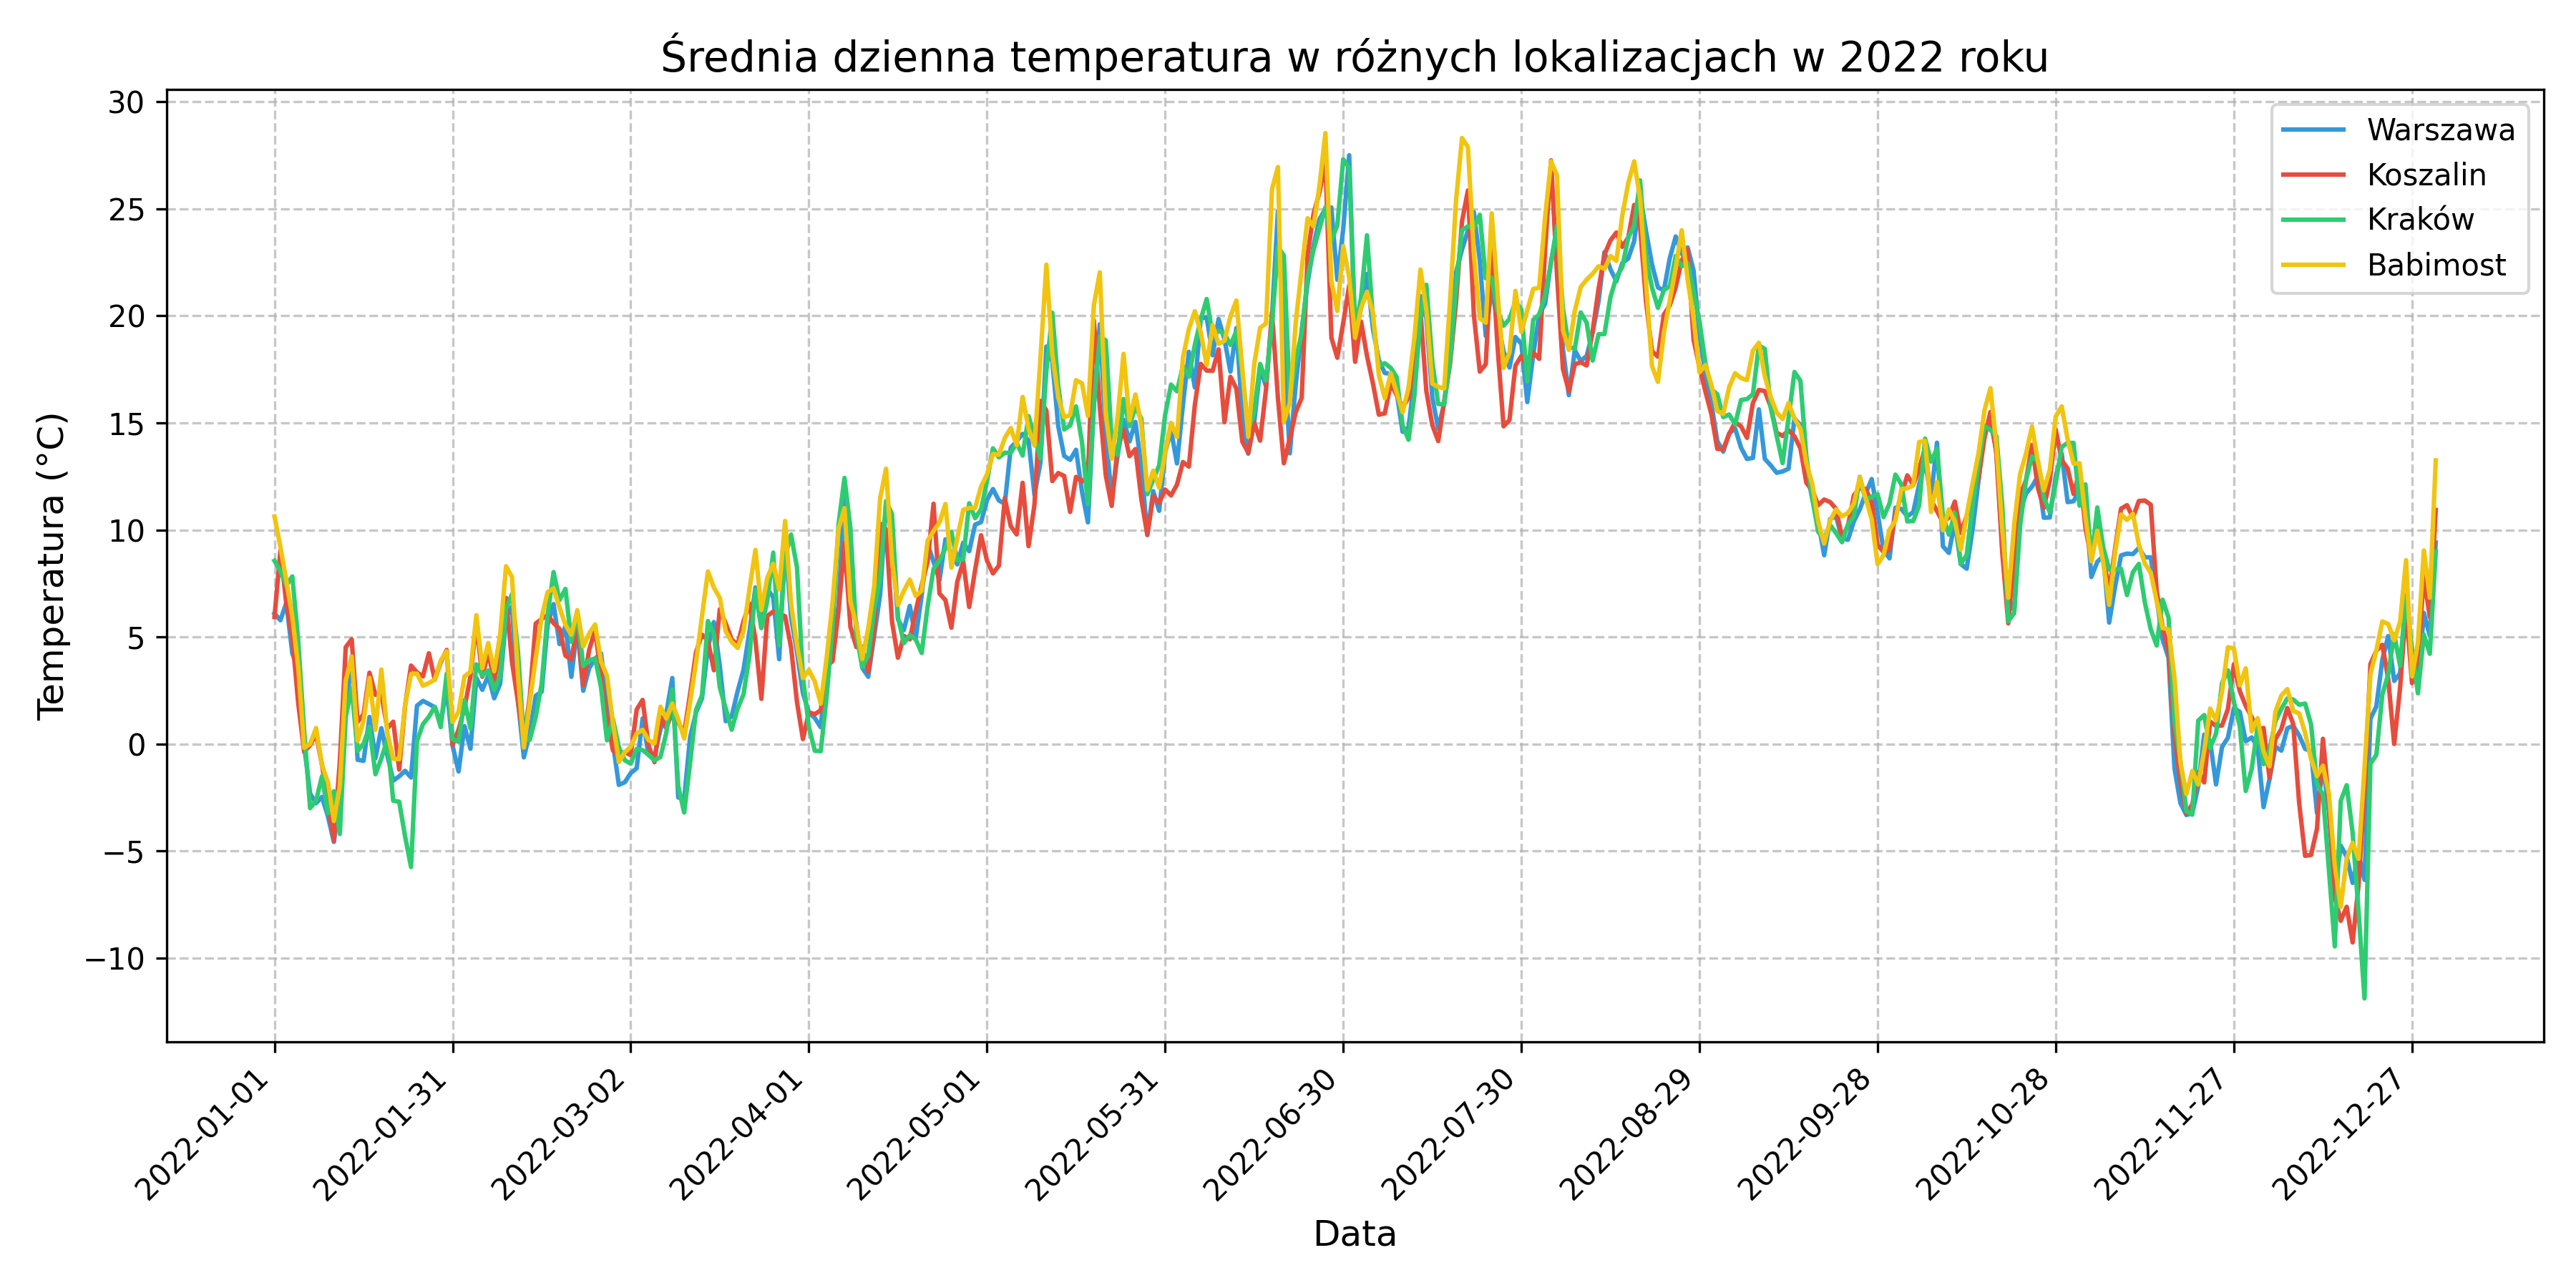
\includegraphics[width=\textwidth]{../plots/data/temp_time_series_2022.png}
    \caption{Zmienność temperatury w czasie (2022)}
    \label{fig:temp-time-series-2022}
\end{figure}

\begin{figure}
    \centering
    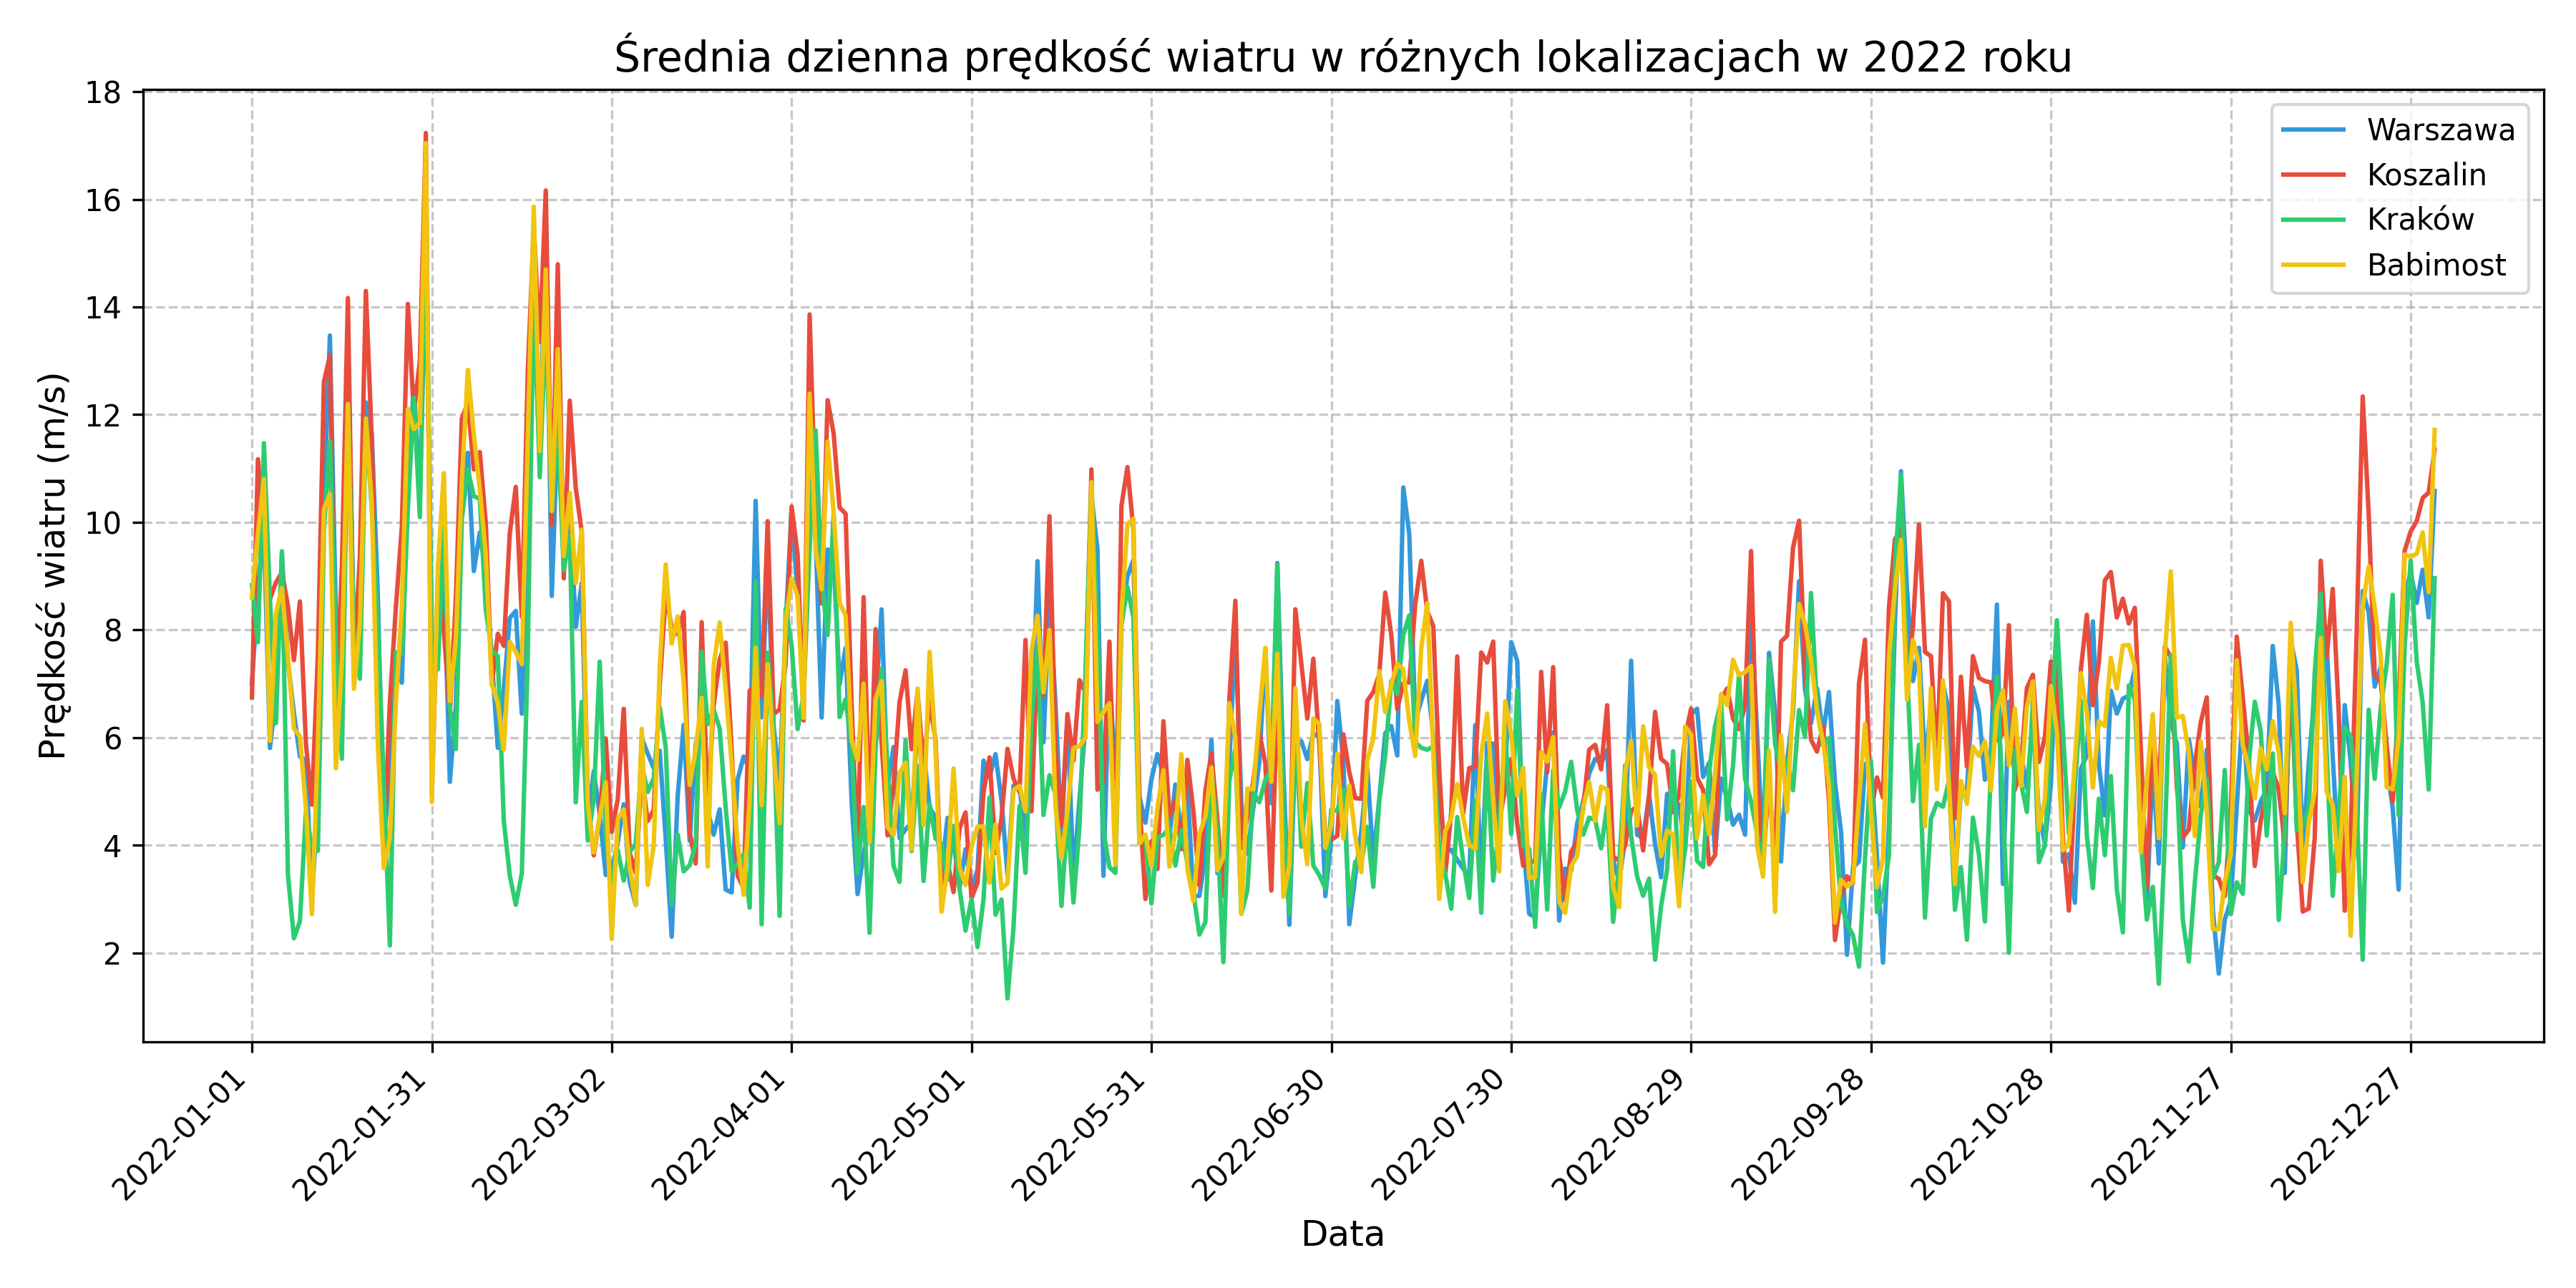
\includegraphics[width=\textwidth]{../plots/data/wind_speed_time_series_2022.png}
    \caption{Zmienność prędkości wiatru w czasie (2022)}
    \label{fig:wind-speed-time-series-2022}
\end{figure}

\begin{figure}
    \centering
    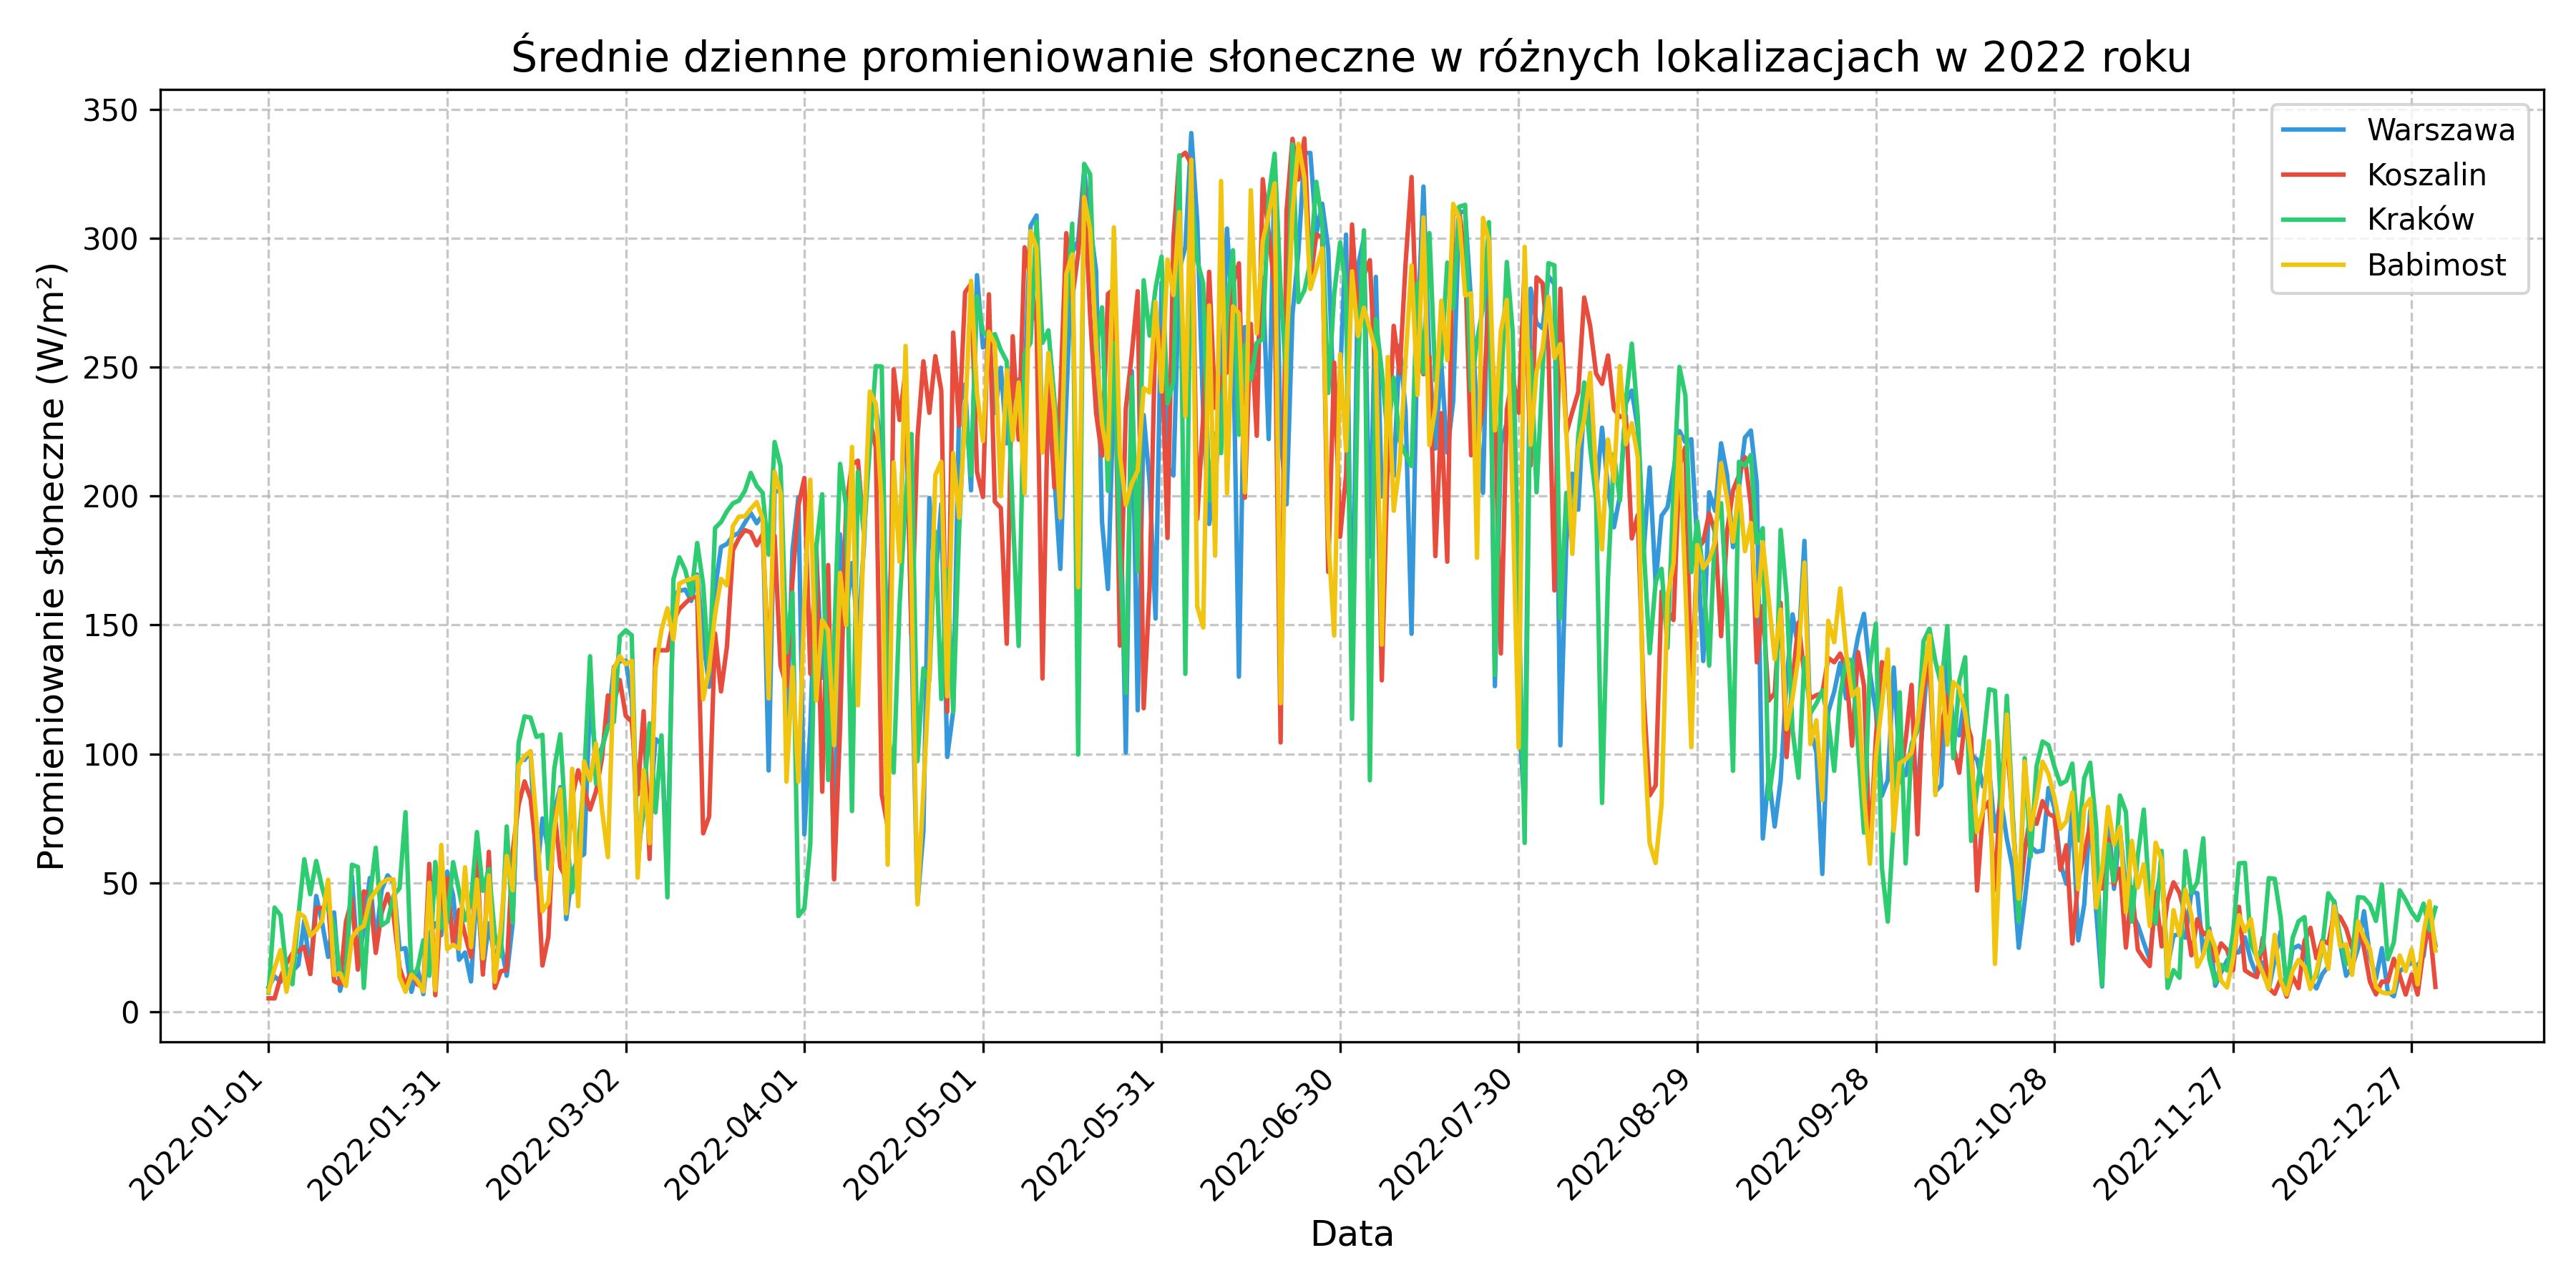
\includegraphics[width=\textwidth]{../plots/data/solar_radiation_time_series_2022.png}
    \caption{Zmienność promieniowania słonecznego w czasie (2022)}
    \label{fig:solar-radiation-time-series-2022}
\end{figure}

\begin{figure}
    \centering
    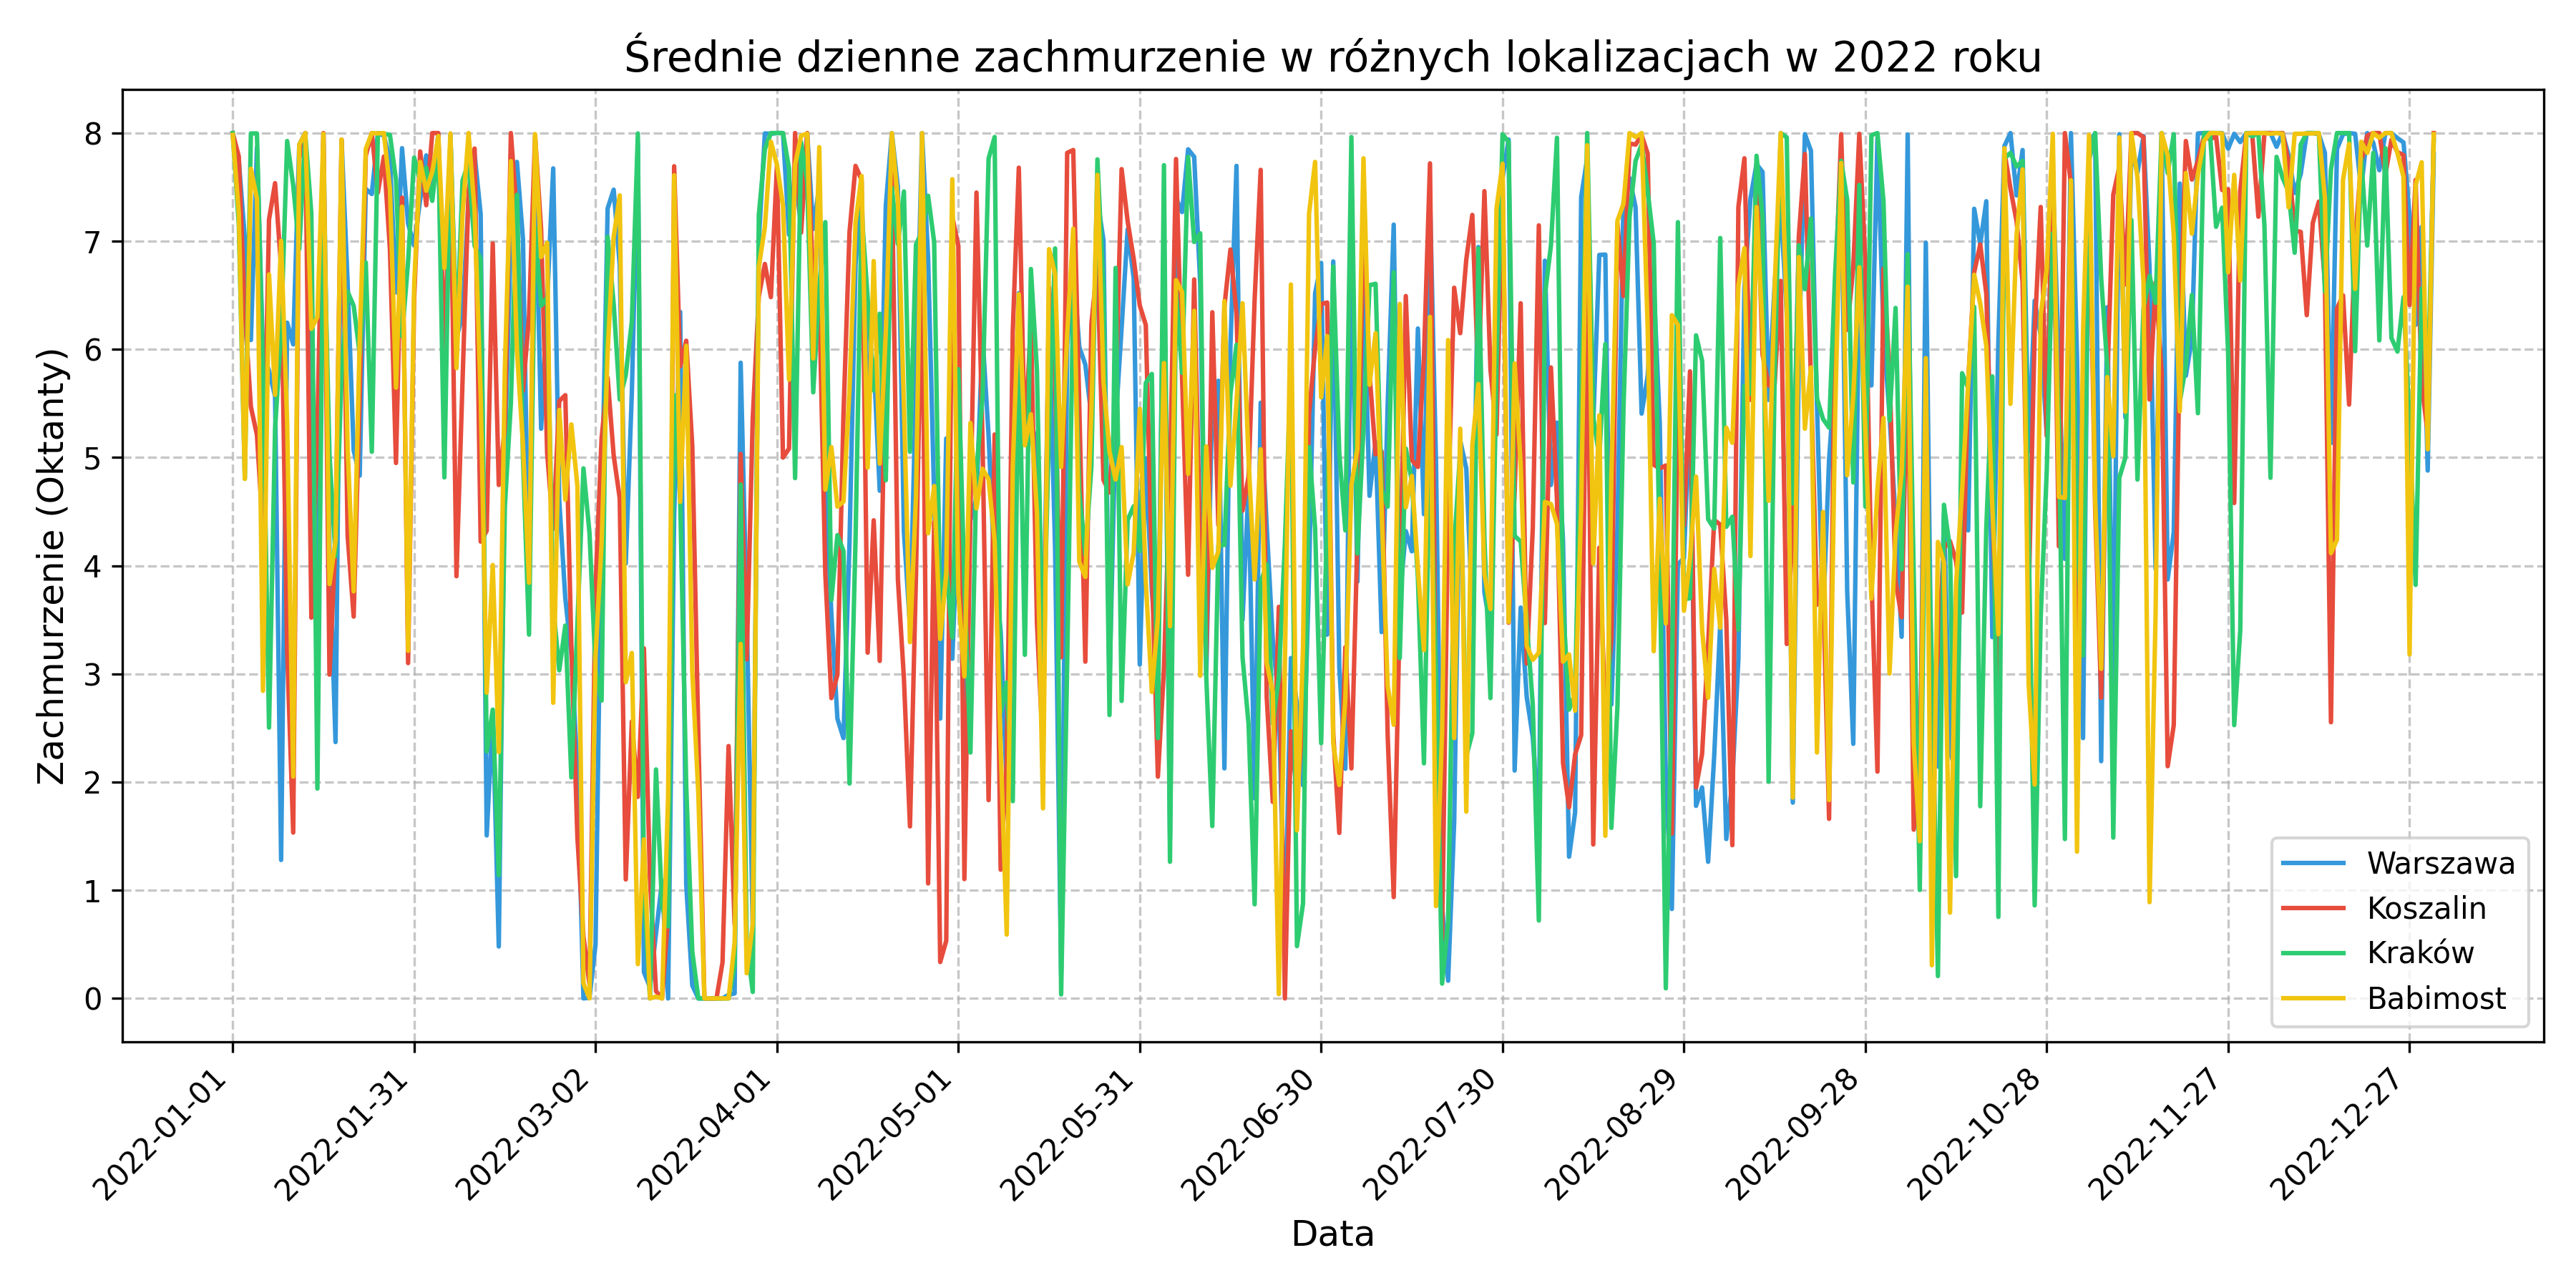
\includegraphics[width=\textwidth]{../plots/data/cloud_cover_time_series_2022.png}
    \caption{Zmienność zachmurzenia w czasie (2022)}
    \label{fig:cloud-cover-time-series-2022}
\end{figure}

W ramach analizy w późniejszej części pracy spróbuję uprościć model i uśrednić wartości parametrów pogodowych dla całego kraju i sprawdzić czy wynik się poprawi. 

\subsection{Produkcja energii z wybranych źródeł}
Zmienne dotyczące produkcji energii z różnych źródeł odgrywają kluczową rolę w analizie cen energii na Rynku Dnia Następnego (RDN), ponieważ odzwierciedlają strukturę podaży energii w Polsce, która ma bezpośredni wpływ na dynamikę cen. W niniejszej pracy uwzględniono osiem zmiennych opisujących produkcję energii: 
\begin{itemize}
    \item \textbf{hard\_coal} - produkcja z węgla kamiennego (MW),
    \item \textbf{coal\_derived} - produkcja z paliw pochodnych węgla (MW),
    \item \textbf{lignite} - produkcja z węgla brunatnego (MW),
    \item \textbf{gas} - produkcja z gazu ziemnego (MW),
    \item \textbf{oil} - produkcja z ropy naftowej lub jej pochodnych (MW),
    \item \textbf{biomass} - produkcja z biomasy (MW),
    \item \textbf{wind} - produkcja z elektrowni wiatrowych lądowych (MW),
    \item \textbf{solar} - produkcja z paneli fotowoltaicznych (MW).
\end{itemize}

Dane te pochodzą z Polskich Sieci Elektroenergetycznych (PSE) i zostały dopasowane do godzinowego formatu danych RDN, co pozwoliło na ich integrację z pozostałymi zmiennymi. 
\begin{figure}[H]
    \centering
    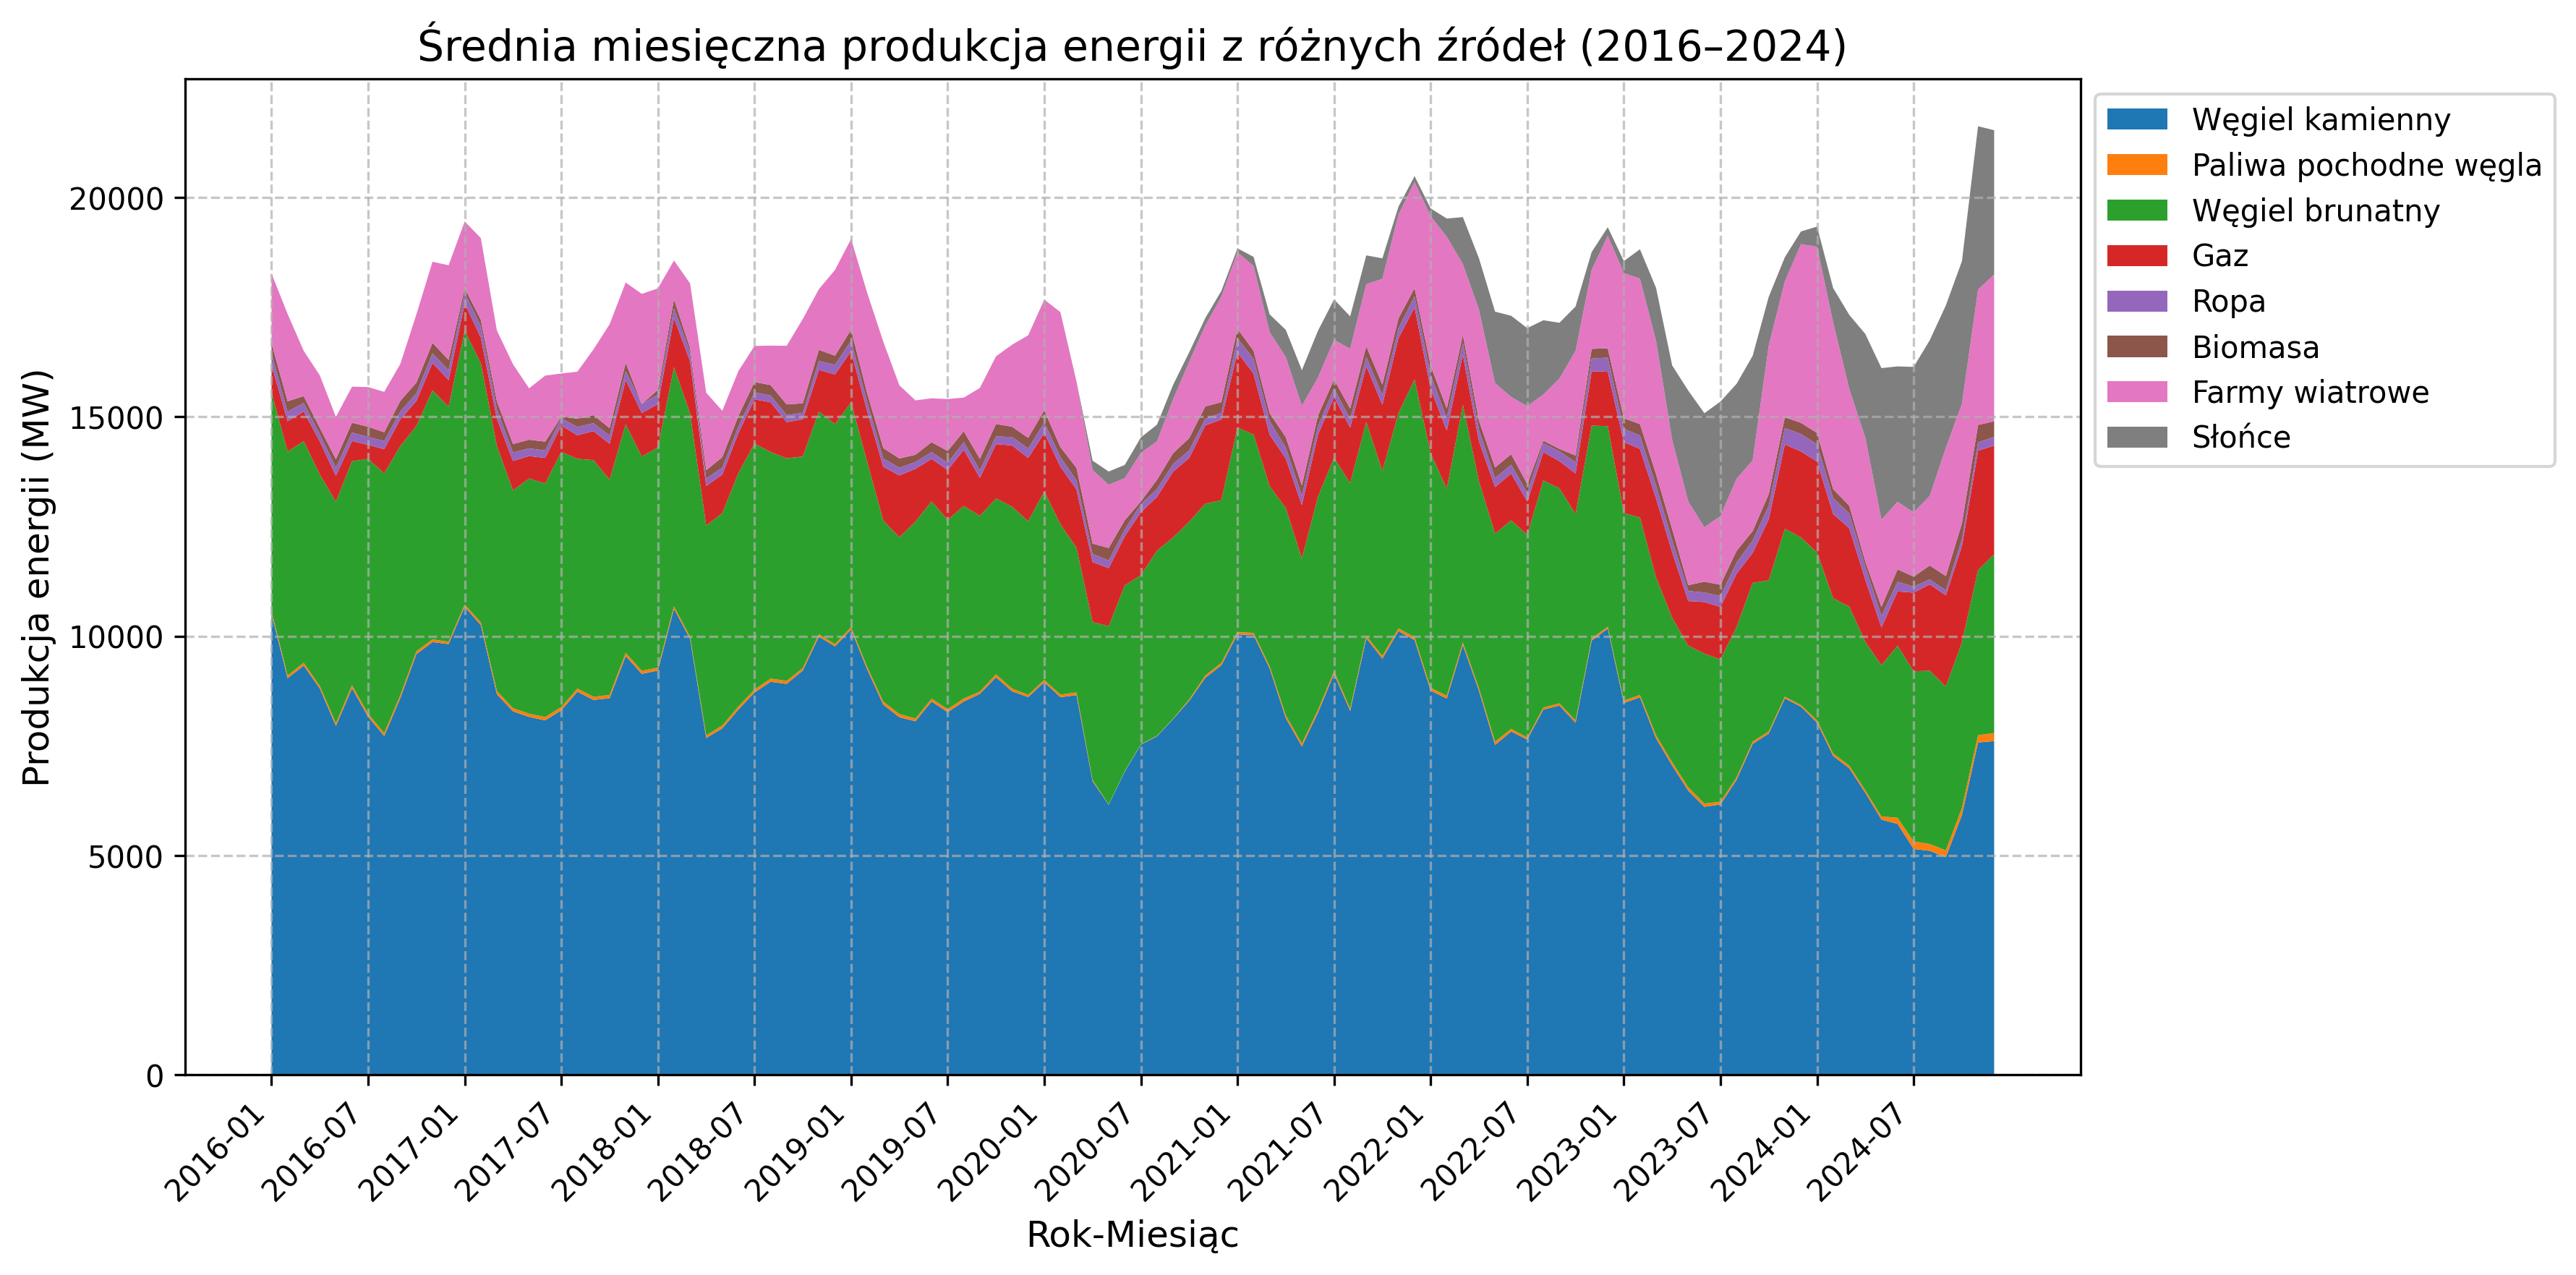
\includegraphics[width=1.1\textwidth]{../plots/data/energy_production_time_series_full.png}
    \caption{Zmienność produkcji energii z różnych źródeł w czasie (2016–2024)}
    \label{fig:energy-production-time-series-full}
\end{figure}

Wykres powyżej przedstawia średnią miesięczną produkcję energii z różnych źródeł w Polsce w latach 2016–2024, co jest istotne w kontekście prognozowania cen energii (EPF) na Rynku Dnia Następnego (RDN). Wykres obszarowy ukazuje dominację węgla kamiennego i brunatnego, której do tej pory odpowiadają za większość produkcji energii elektrycznej. Biomasa oraz paliwa pochodne węgla stanowią znikomą część podaży i mogą być pominięte dla redukcji ilości zmiennych. Produkcja za pomocą gazu i ropy stale posiada niewielką, ale istotną część produkcji energii. Warto zauważyć, że produkcja z OZE, szczególnie ze słońca znacząco rośnie w ostatnich latach, co może mieć istotny wpływ na ceny energii i umiejętność jej prognozowania. W najbardziej korzystne dla gospodatki momenty część produkcji z OZE może przekraczać zapewnienie energii z węgla, co może prowadzić do spadku cen energii. Warto również zauważyć, że produkcja z węgla kamiennego i brunatnego jest bardziej stabilna i przewidywalna niż produkcja z OZE, co może wpływać na dokładność prognoz. W związku z tym, zmienne dotyczące produkcji energii z różnych źródeł są istotnym elementem analizy i modelowania cen energii na RDN.

\subsection{Handel energią z państwami sąsiednimi}
Zmienne dotyczące wymiany energii z innymi krajami są istotnym elementem analizy cen energii na Rynku Dnia Następnego (RDN), ponieważ pozwalają na uwzględnienie wpływu handlu międzynarodowego na ceny energii w Polsce. W niniejszej pracy uwzględniono następujące zmienne opisujące wymianę energii z innymi krajami:
